\documentclass[12pt, a4paper]{article}
\usepackage{ctex} % 支持中文处理
\usepackage{geometry} % 页面布局
\usepackage{graphicx} % 图片支持
\usepackage{subcaption}
\usepackage{hyperref} % 超链接支持
\usepackage{amsmath} % 数学公式
\usepackage{amsfonts}
\usepackage{amssymb}
\usepackage{amsthm}
\usepackage{bm}
\usepackage{color}

\geometry{left=2.5cm,right=2.5cm,top=2.5cm,bottom=2.5cm} % 设置页边距
\title{结果讨论}
\author{安庭毅\ 工学院 \ 2100011014}
\date{\today} % 使用今天的日期

\begin{document}

\maketitle % 显示标题
\section{计算域设置及网格数影响}
在本次作业中,计算域统一设置为$[-0.5,0.5]$,时间推进到Sod激波管问题的典型时间T=0.2。这样设置的时空设置既保证了空间的对称性,也确保了激波和疏散波在设置的时间内不会传递至边界,避免了计算域截断的反射问题。
在计算过程中,需用到的边界条件可以通过根据选用的计算格式设置相应数目的Ghost Cell来确定。换言之,对于Ghost Cell,不用计算该节点的通量导数,只需将其设置为0。在时间推进中,节点处的守恒量不发生变化。

网格数影响了激波捕捉的分辨率。越细密的网格,对激波捕捉越精确,间断处的厚度越小;反之,粗格点带来的数值耗散效应更强,间断区过渡被平滑化。这在本次作业中选用的Roe格式计算结果中十分明显,如图1所示。
\begin{figure}[htbp]
    \centering
    \begin{subfigure}[b]{0.45\textwidth} 
        \centering
        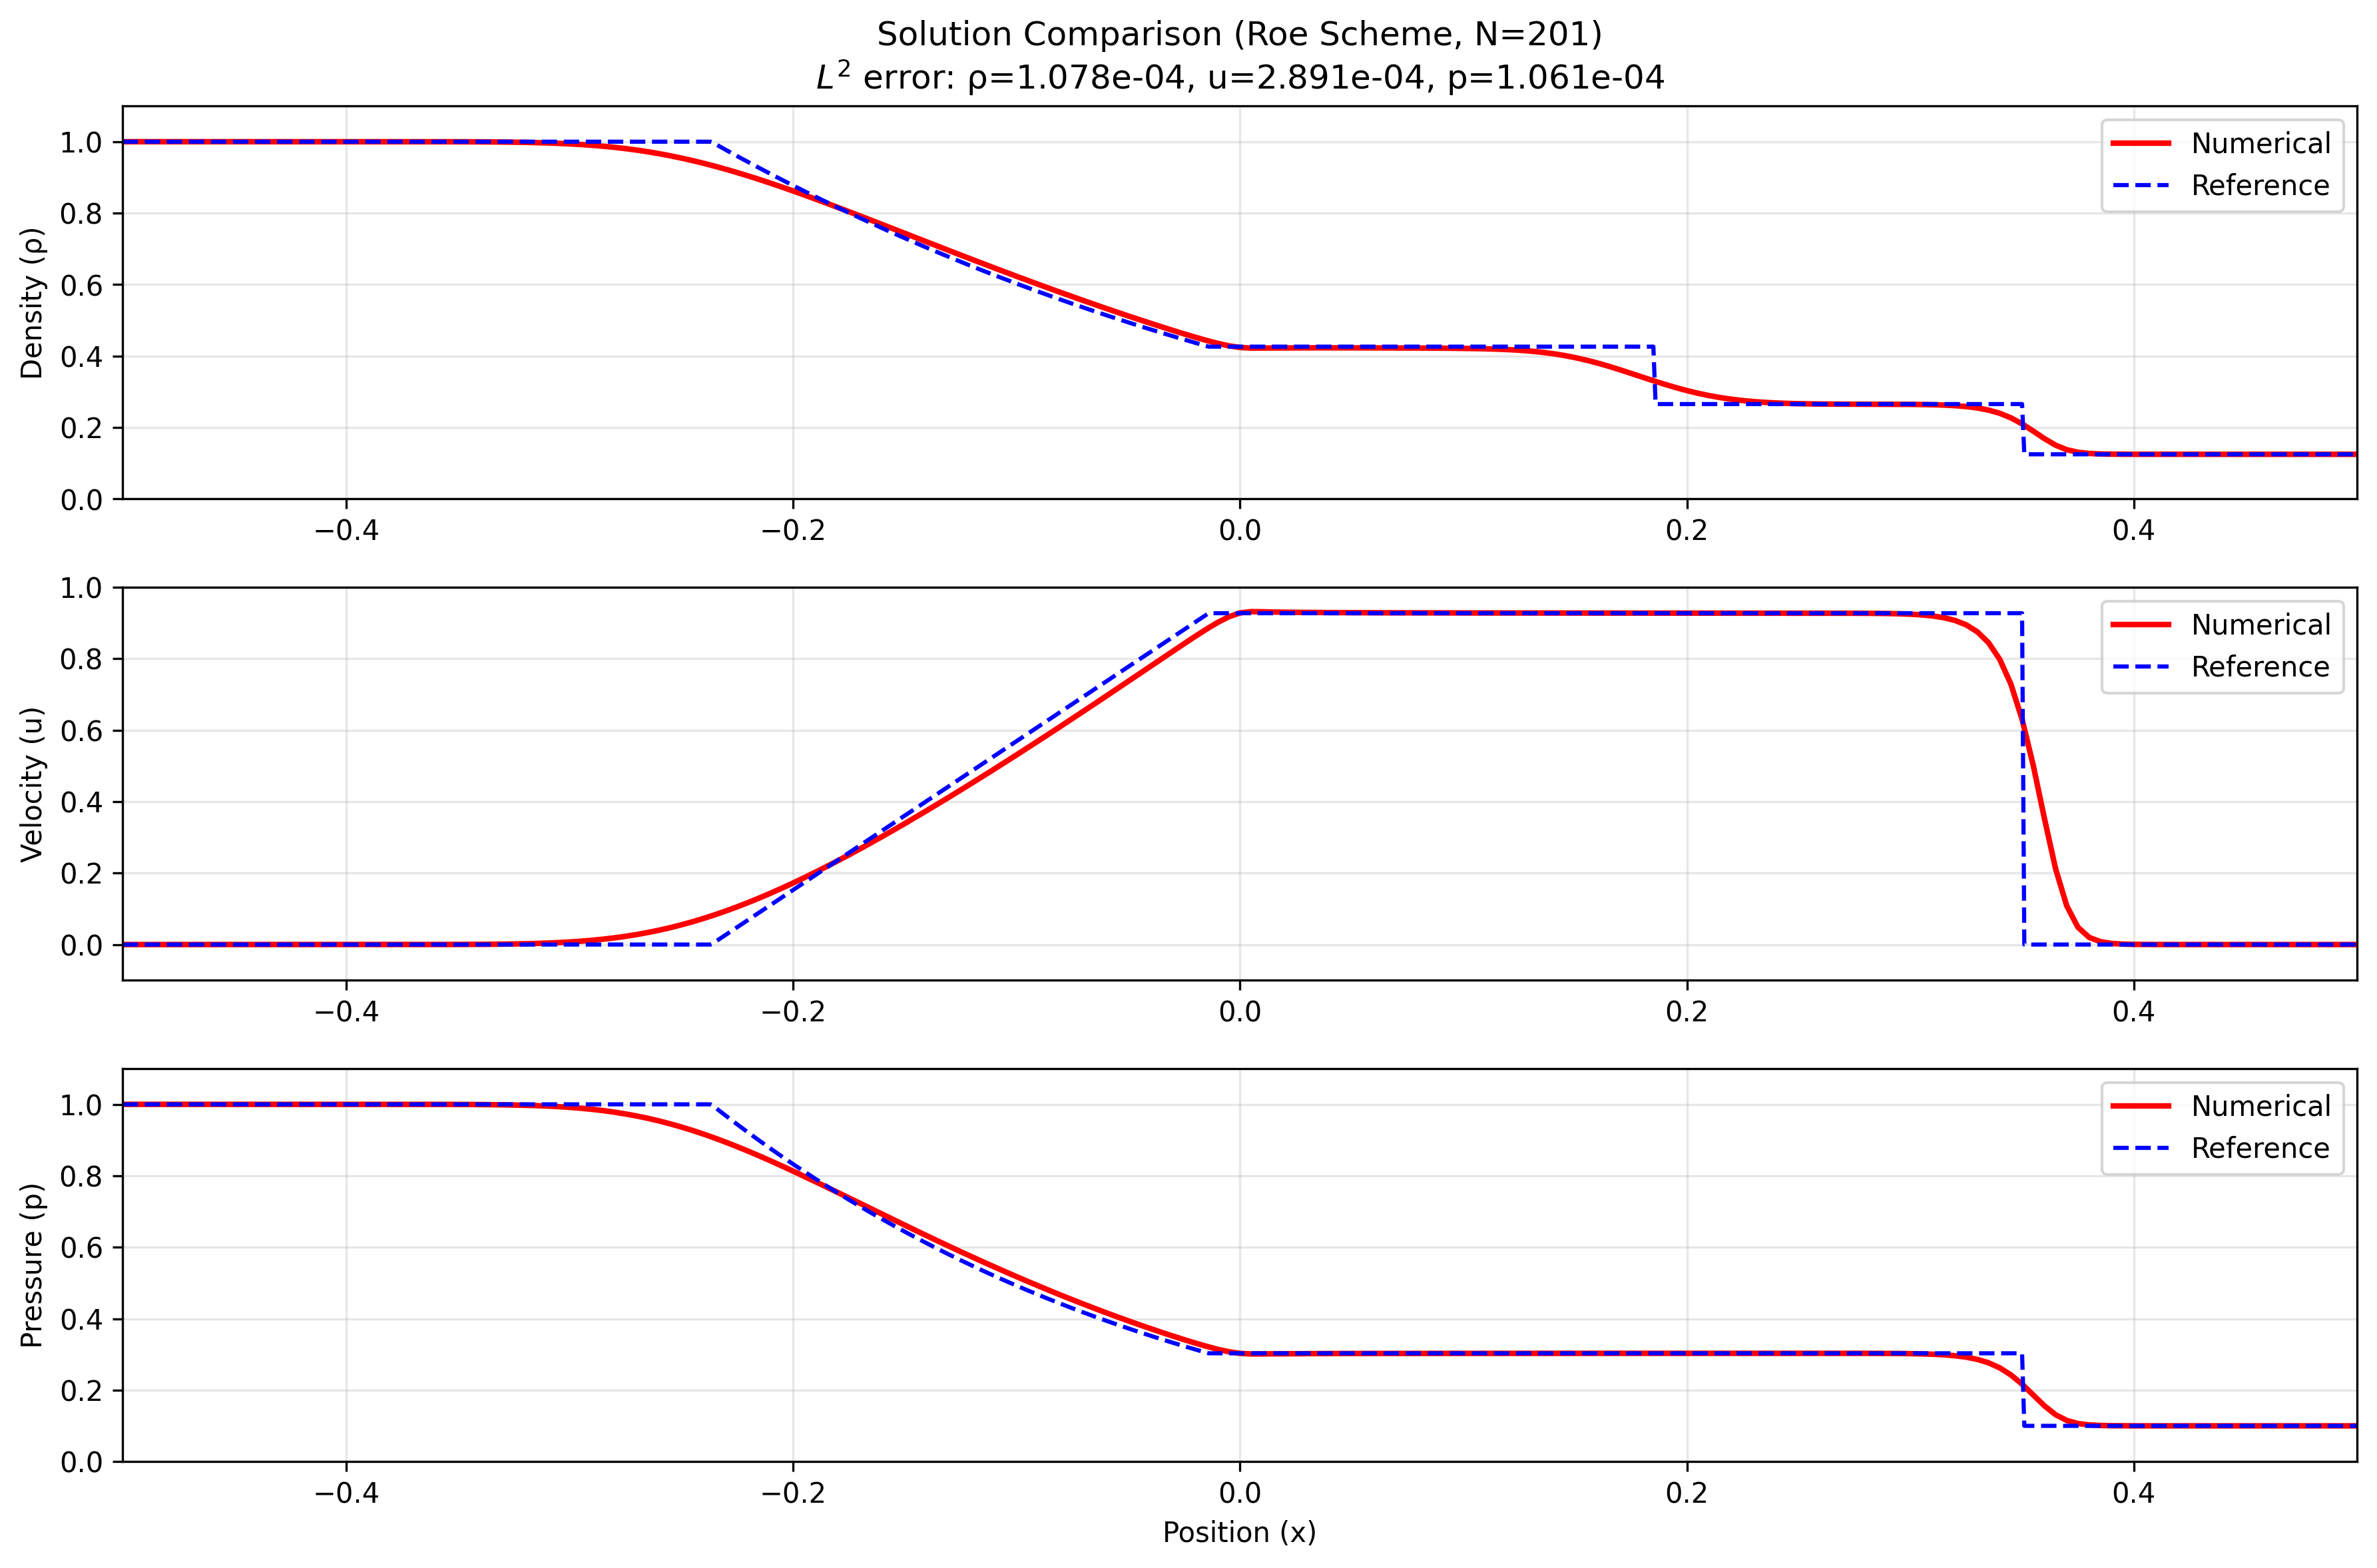
\includegraphics[width=\textwidth]{./pictures/Solution Comparison (Roe Scheme, N=201).png} 
        \caption{Roe格式,N=201}
    \end{subfigure}
    \hfill
    \begin{subfigure}[b]{0.45\textwidth} 
        \centering
        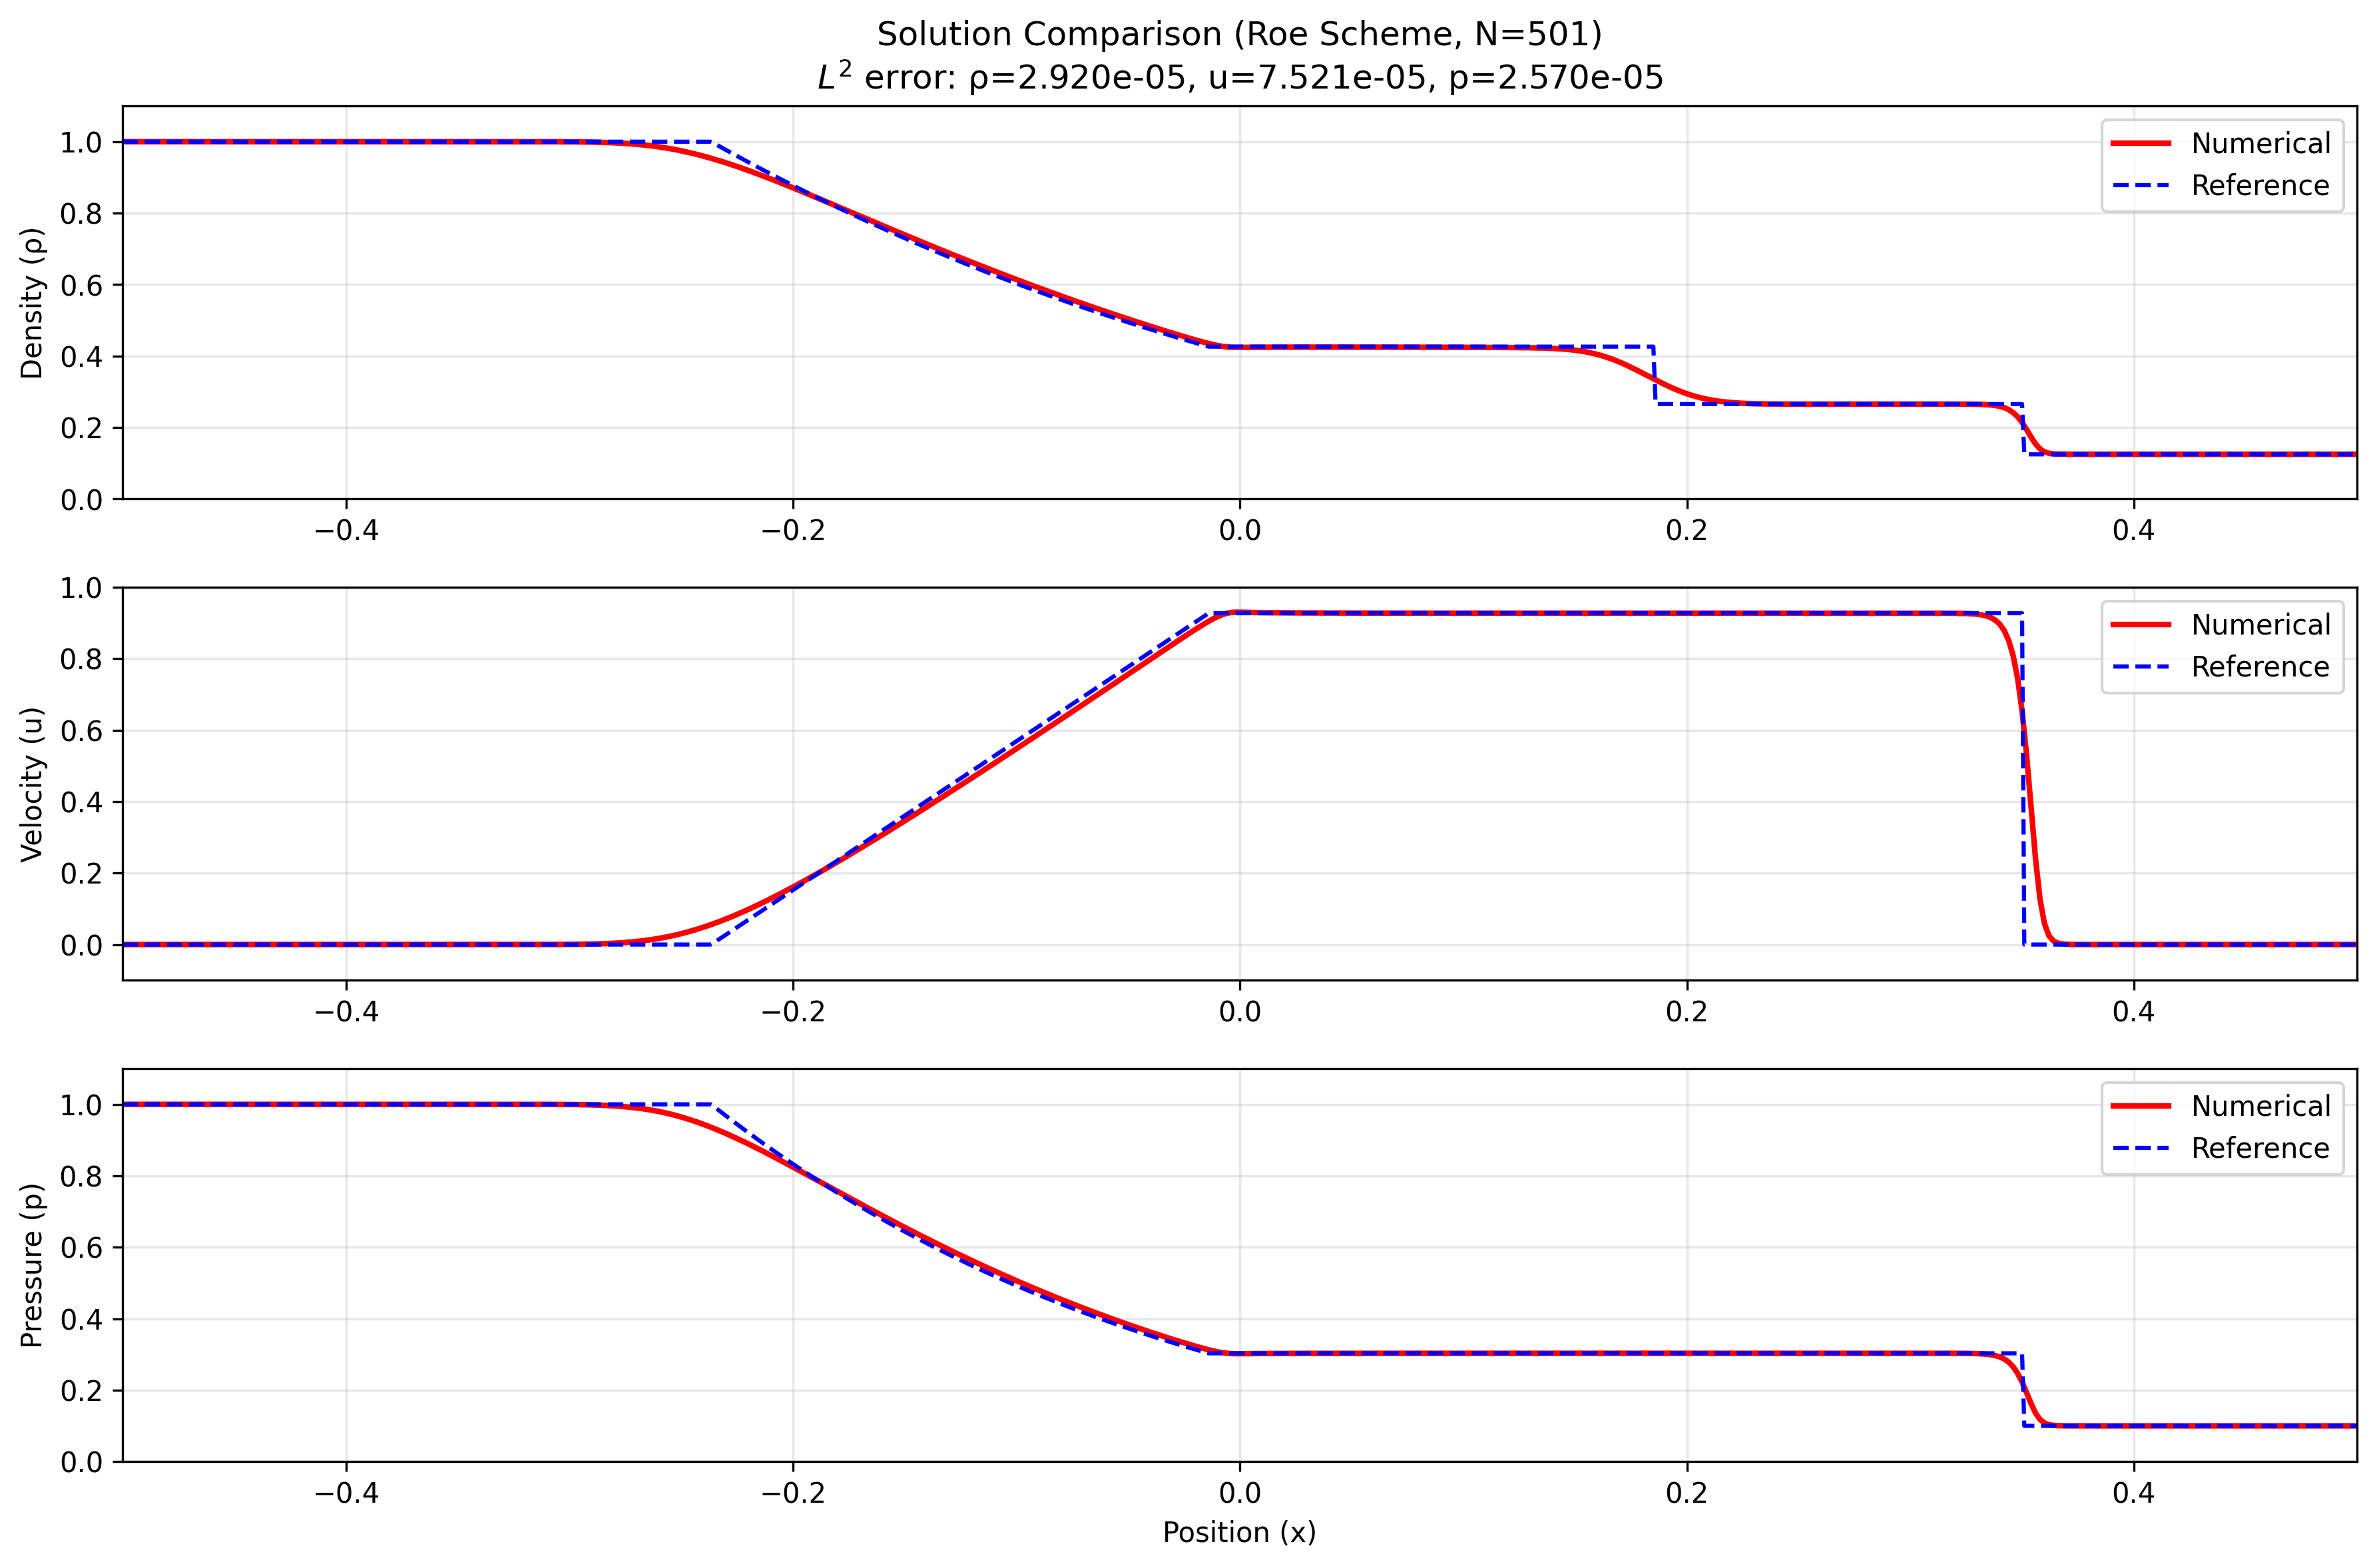
\includegraphics[width=\textwidth]{./pictures/Solution Comparison (Roe Scheme, N=501).png} 
        \caption{Roe格式,N=501}
    \end{subfigure}
    \vspace{0.5cm}
    \centering
    \begin{subfigure}[b]{0.45\textwidth} 
        \centering
        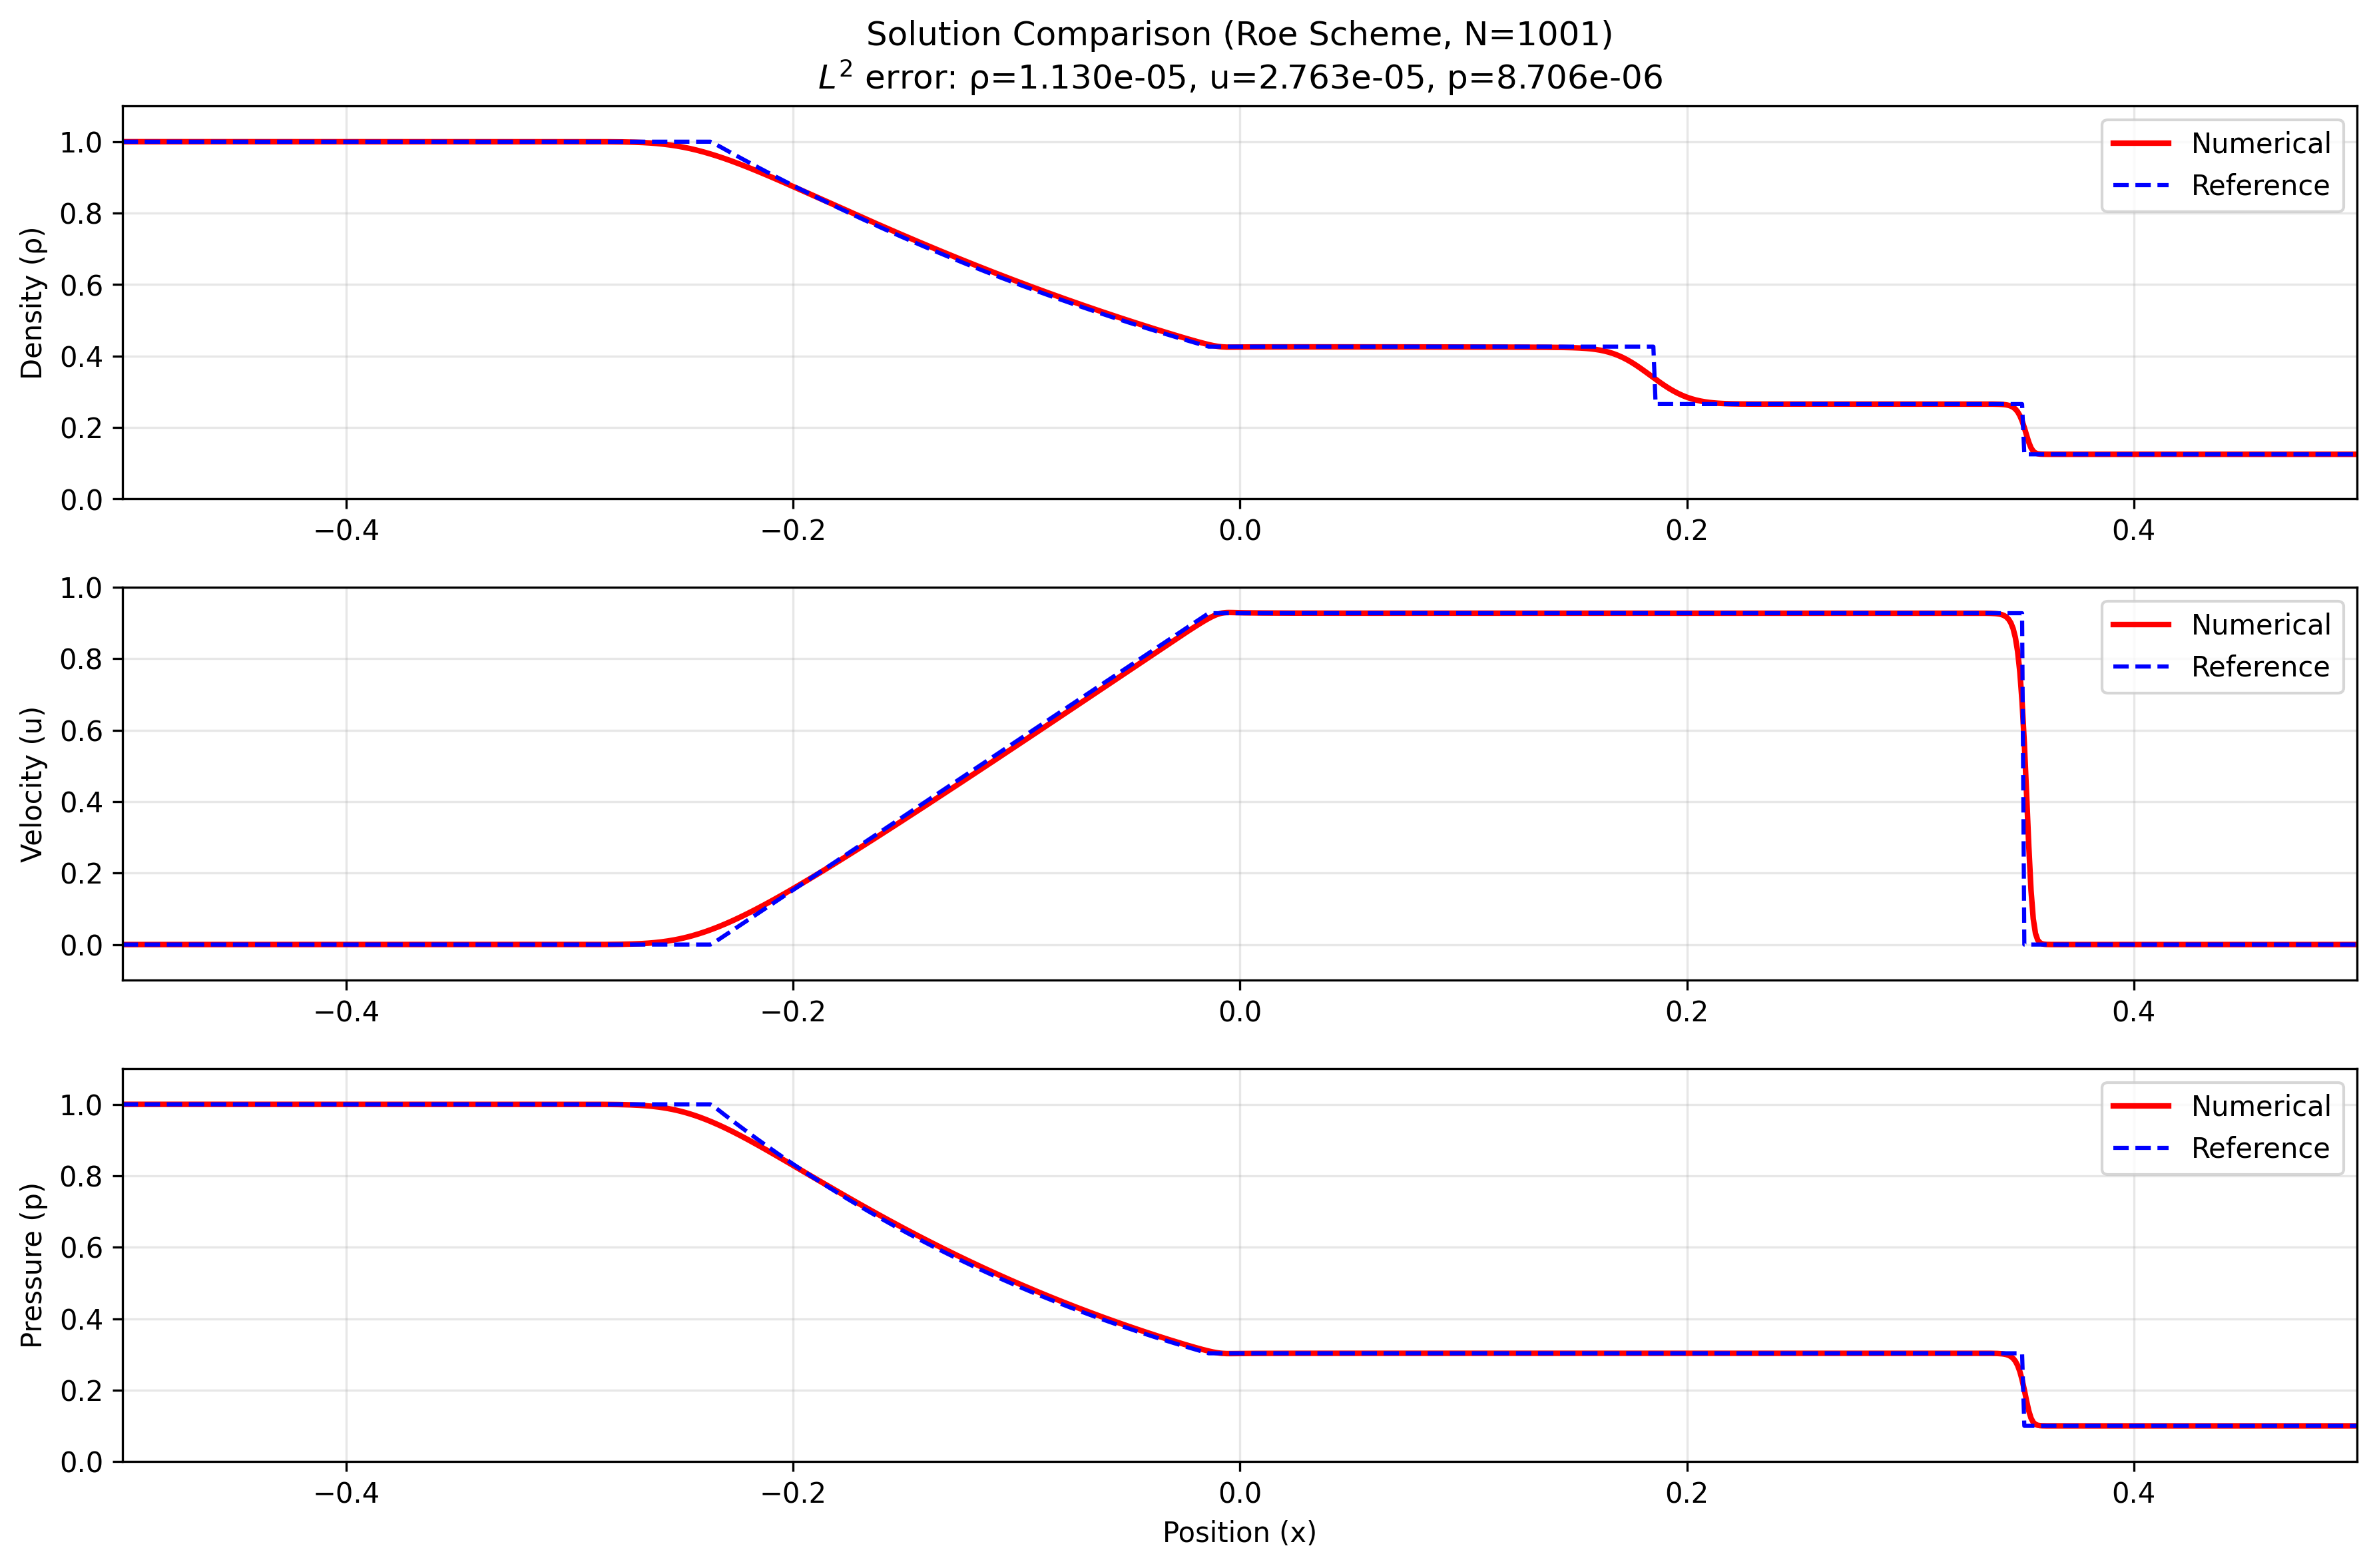
\includegraphics[width=\textwidth]{./pictures/Solution Comparison (Roe Scheme, N=1001).png} 
        \caption{Roe格式,N=1001}
    \end{subfigure}
    \hfill
    \begin{subfigure}[b]{0.45\textwidth} 
        \centering
        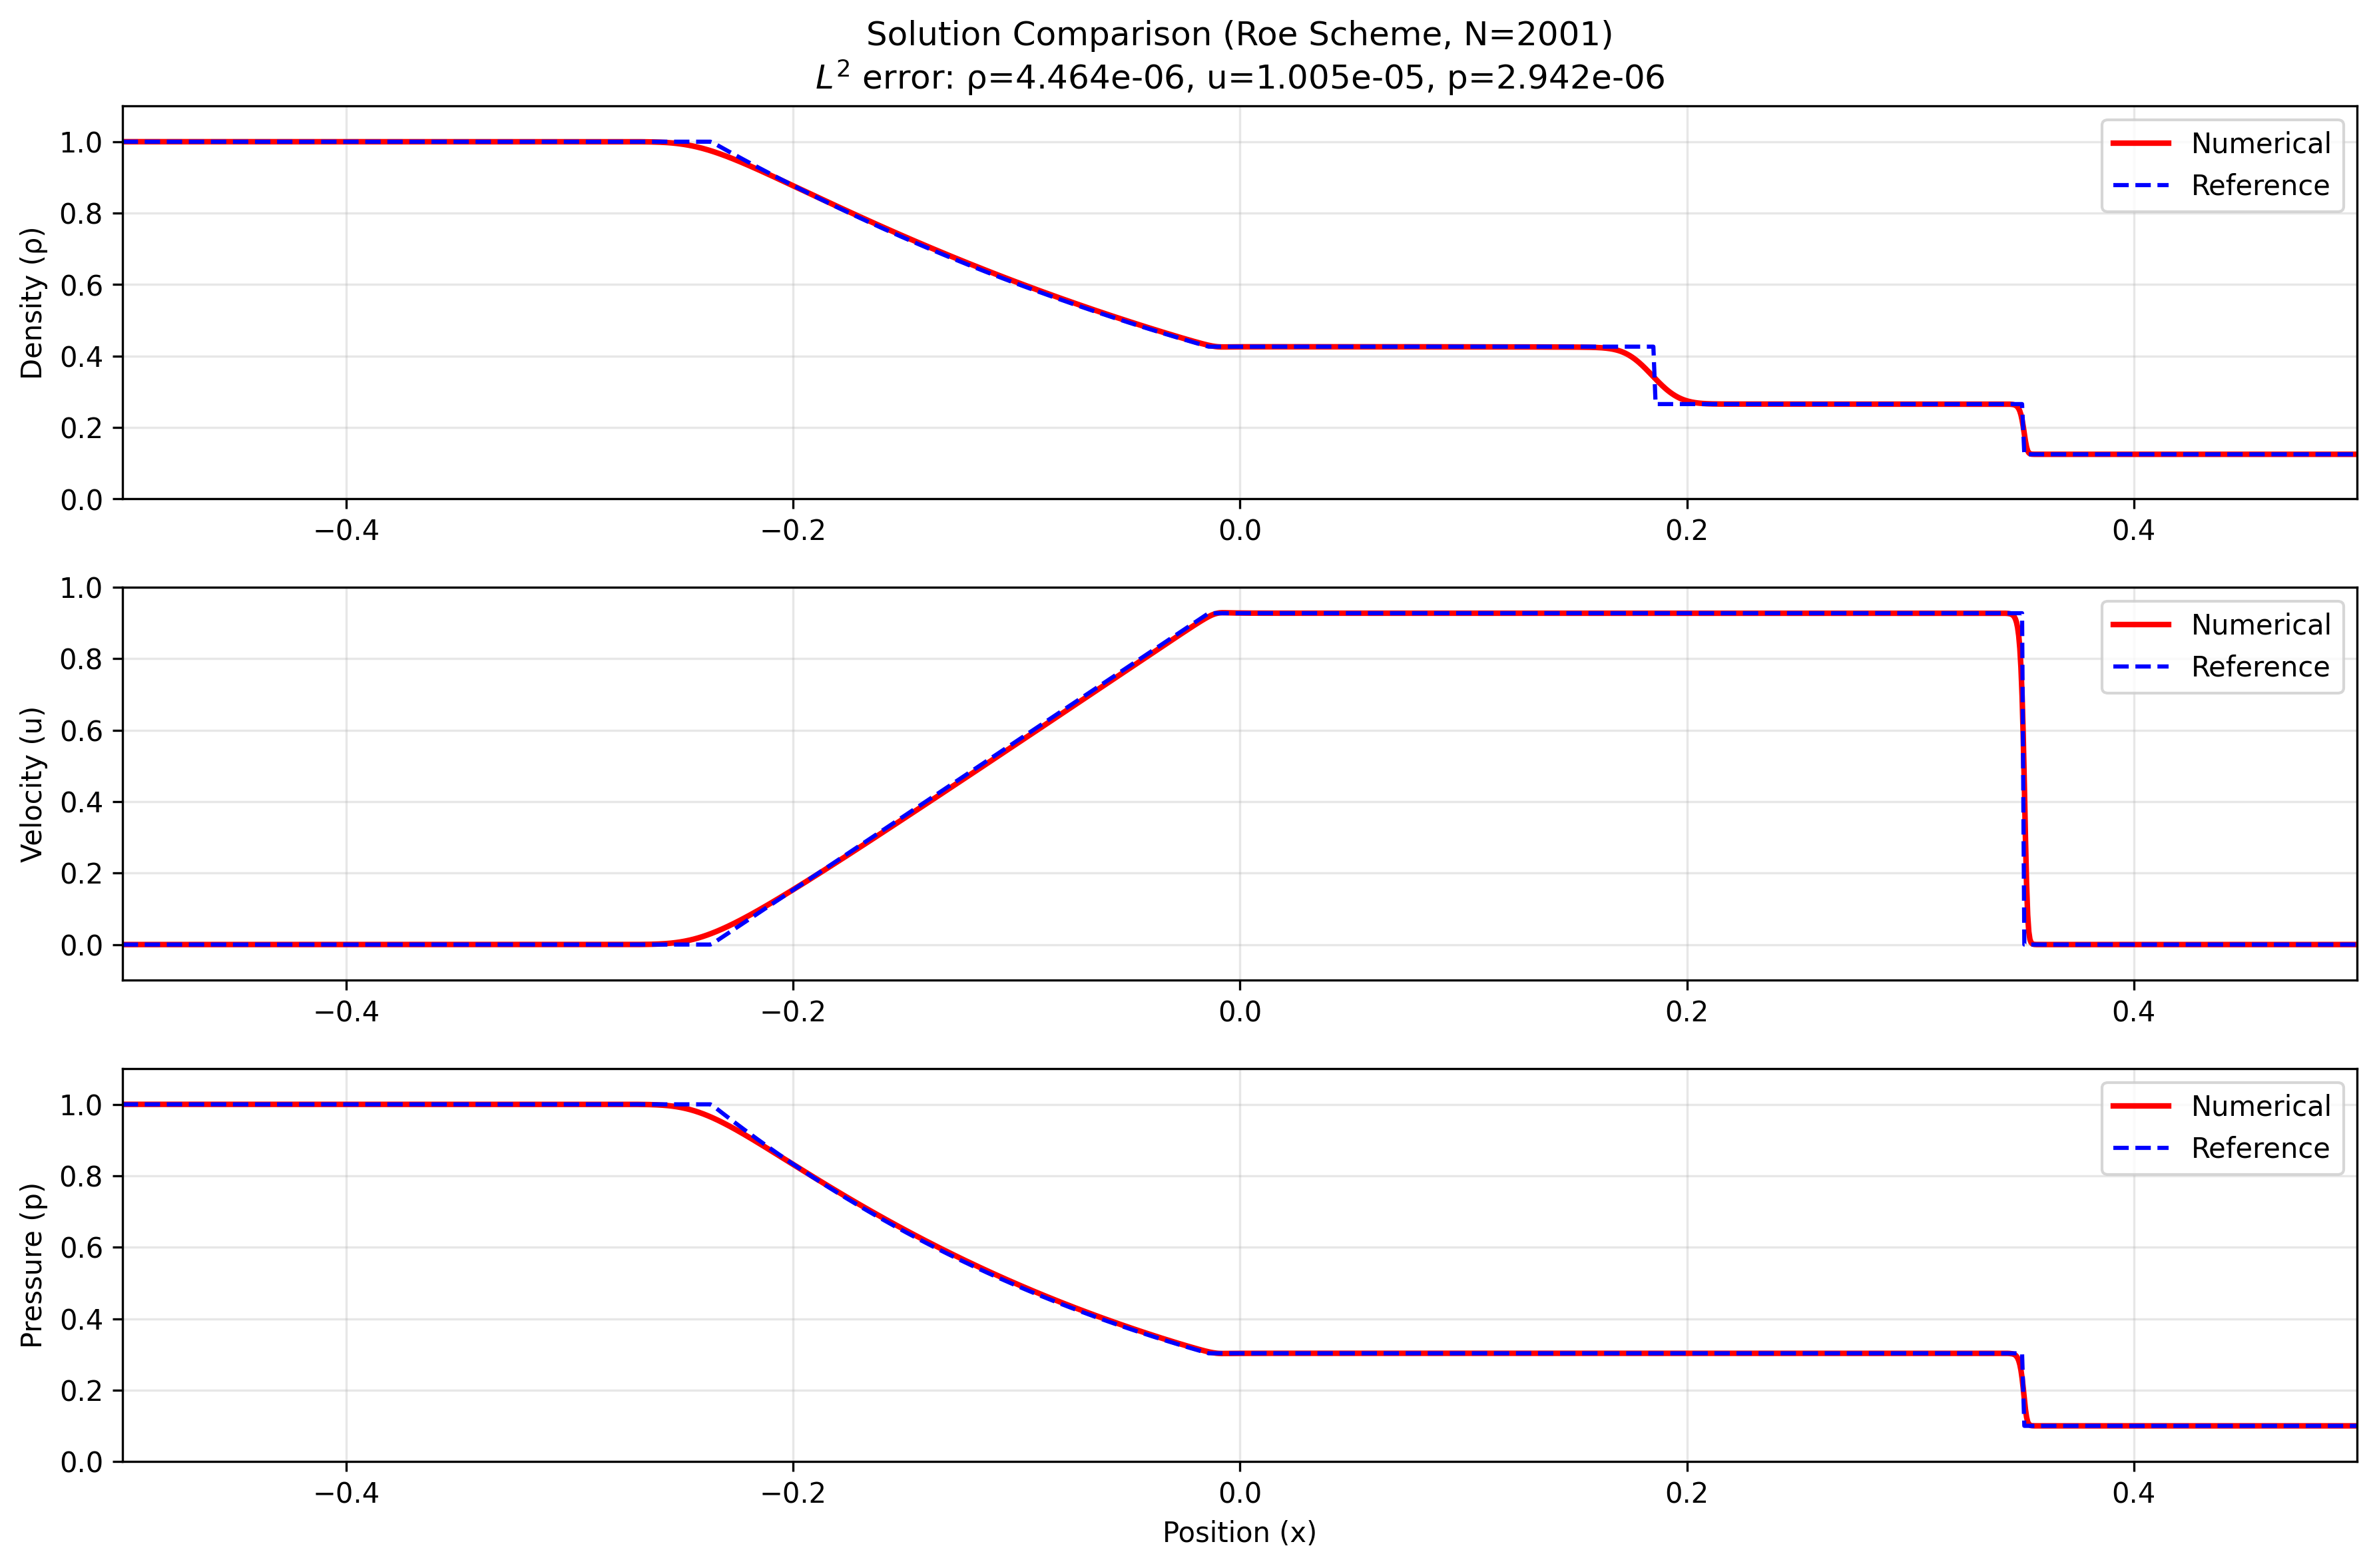
\includegraphics[width=\textwidth]{./pictures/Solution Comparison (Roe Scheme, N=2001).png} 
        \caption{Roe格式,N=2001}
    \end{subfigure}
    \caption{Roe格式在不同网格数设置下的计算结果}
\end{figure}

之所以Roe格式的耗散效应对空间网格密度如此敏感,应当是因为在确定左右状态时直接取用了一节迎风格式,以节点处的值直接确定状态。这带来了较强的数值耗散。如果采用其他形式的格式确定左右状态,耗散效应应能降低。

考虑到计算效率和激波捕捉精度的平衡,本次作业中的格式均采用N=1001作为网格数。

\section{TVD格式计算结果}
TVD格式采用三种不同限制器给出的计算结果如图2所示。
\begin{figure}[htbp]
    \centering
    \begin{subfigure}[b]{0.45\textwidth} 
        \centering
        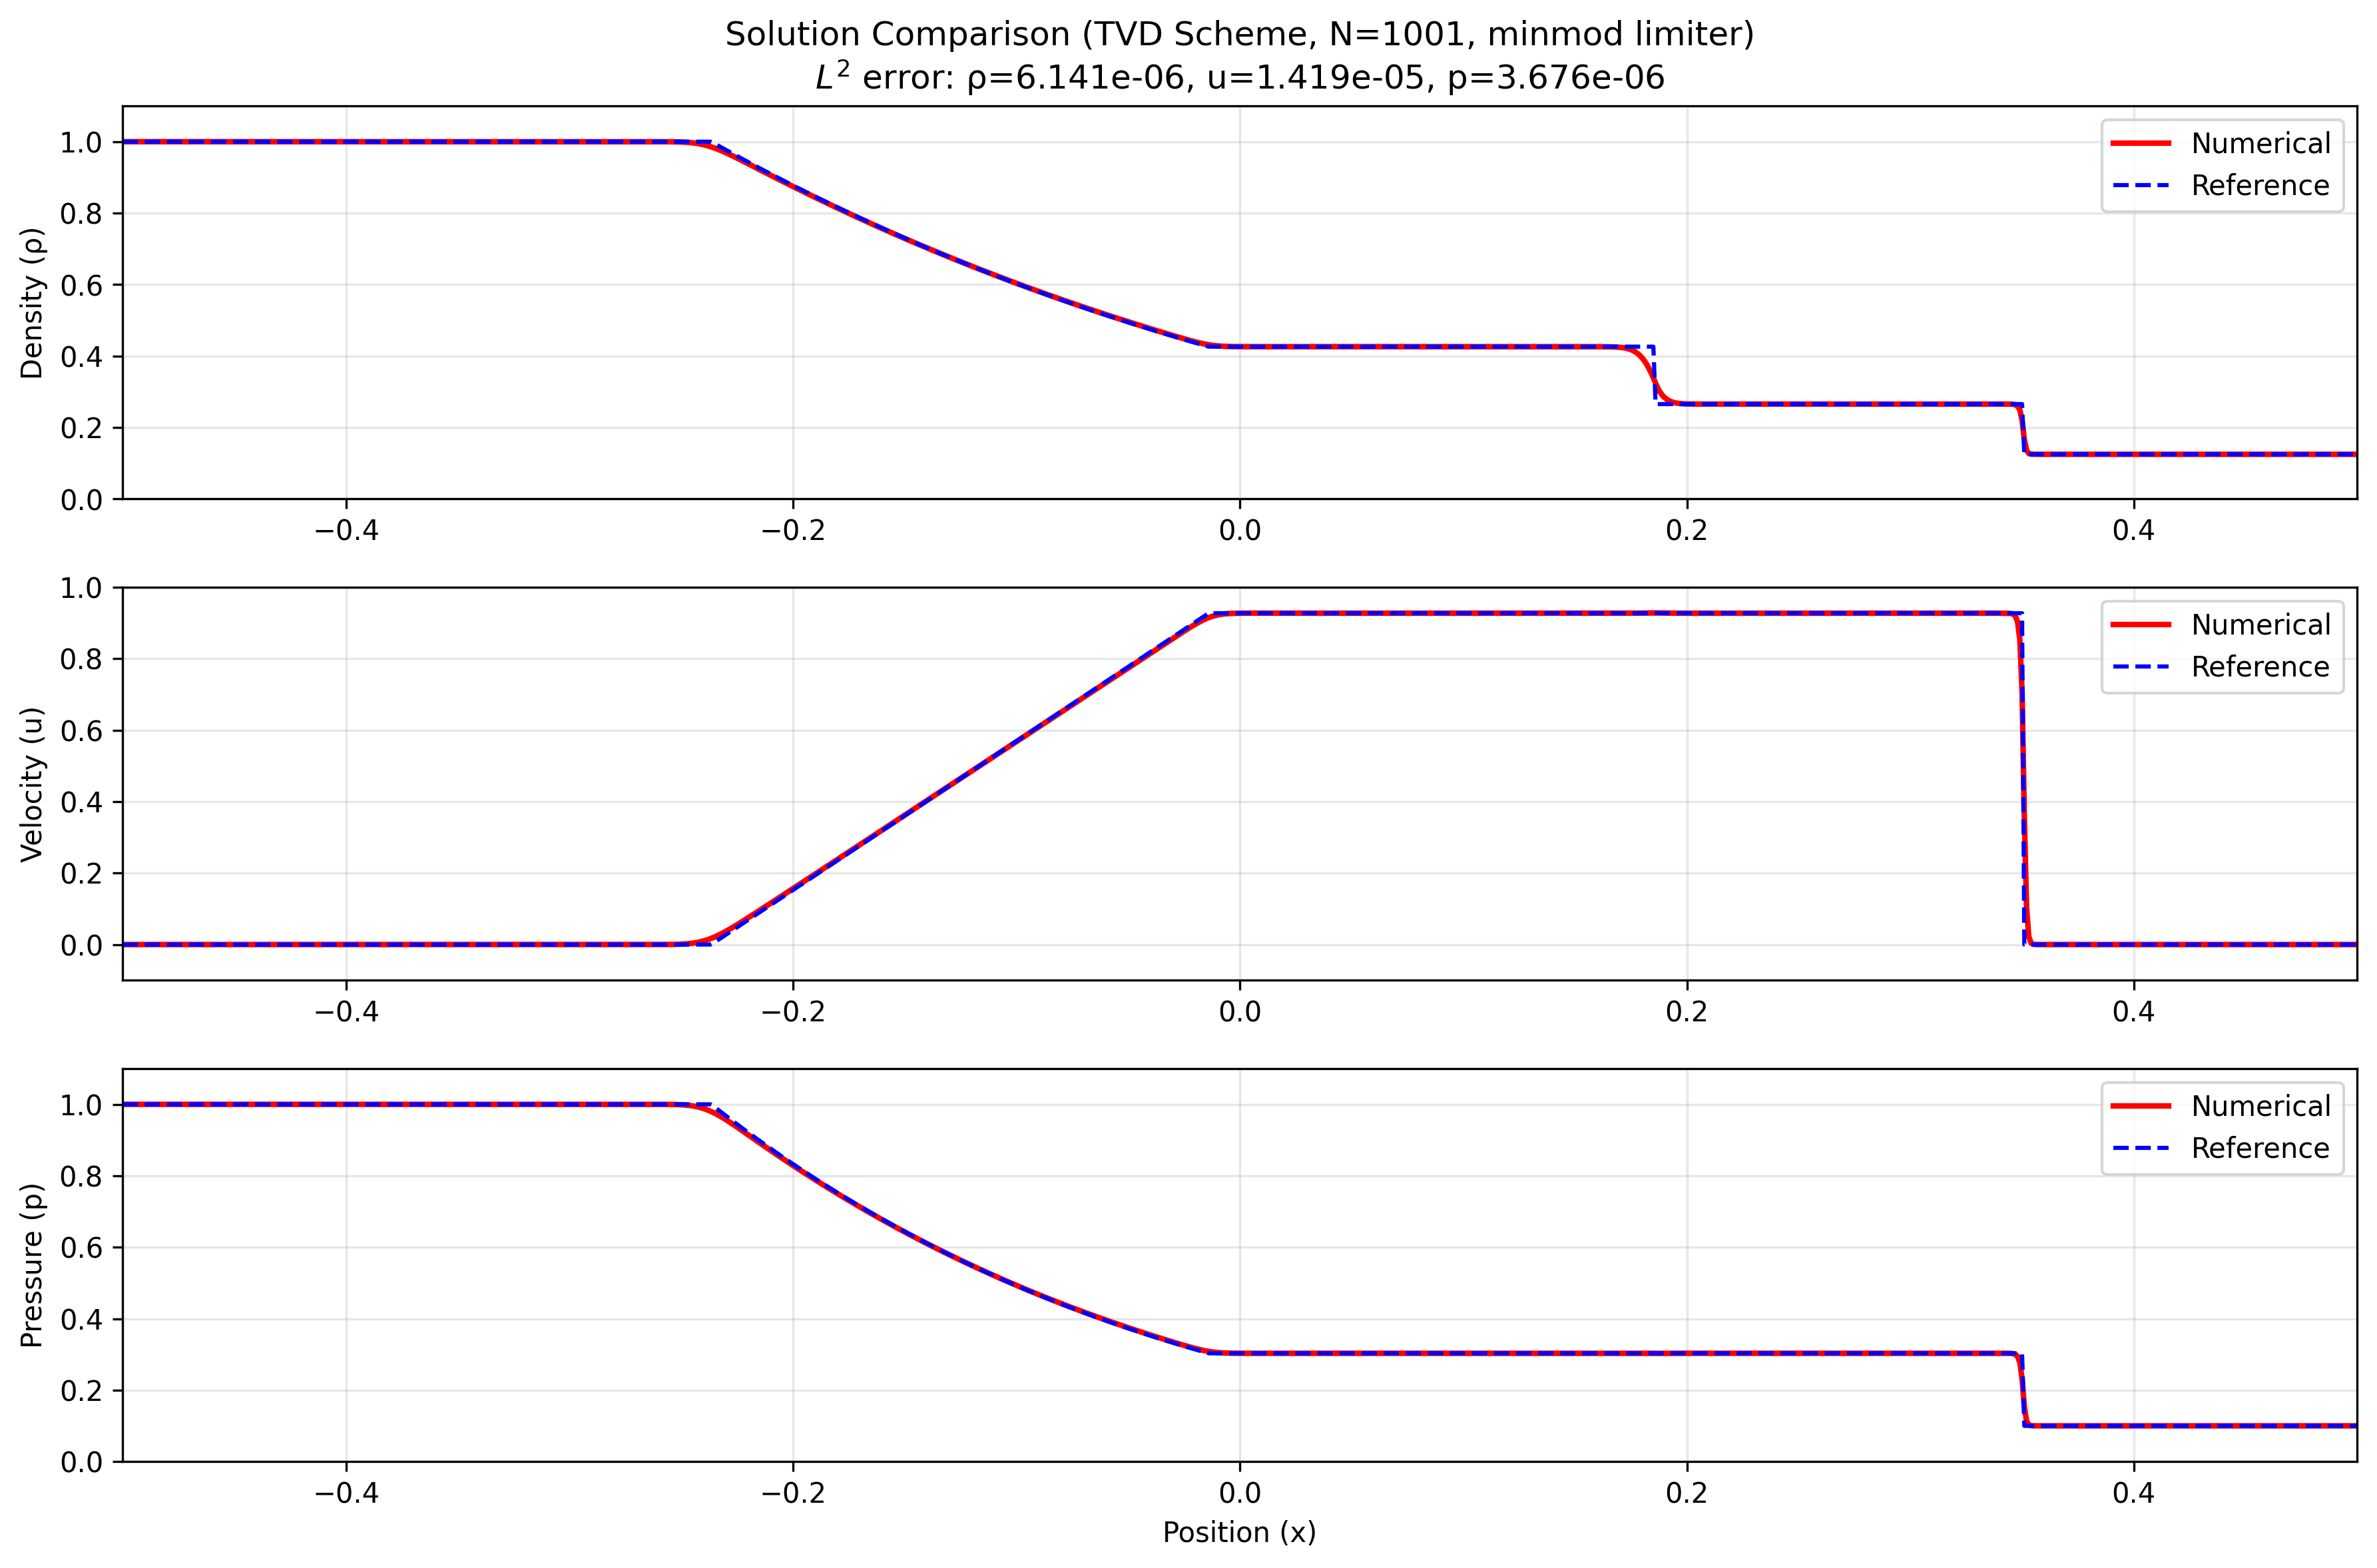
\includegraphics[width=\textwidth]{./pictures/Solution Comparison (TVD Scheme, N=1001, minmod limiter).png} 
        \caption{Minmod限制器}
    \end{subfigure}
    \hfill
    \begin{subfigure}[b]{0.45\textwidth} 
        \centering
        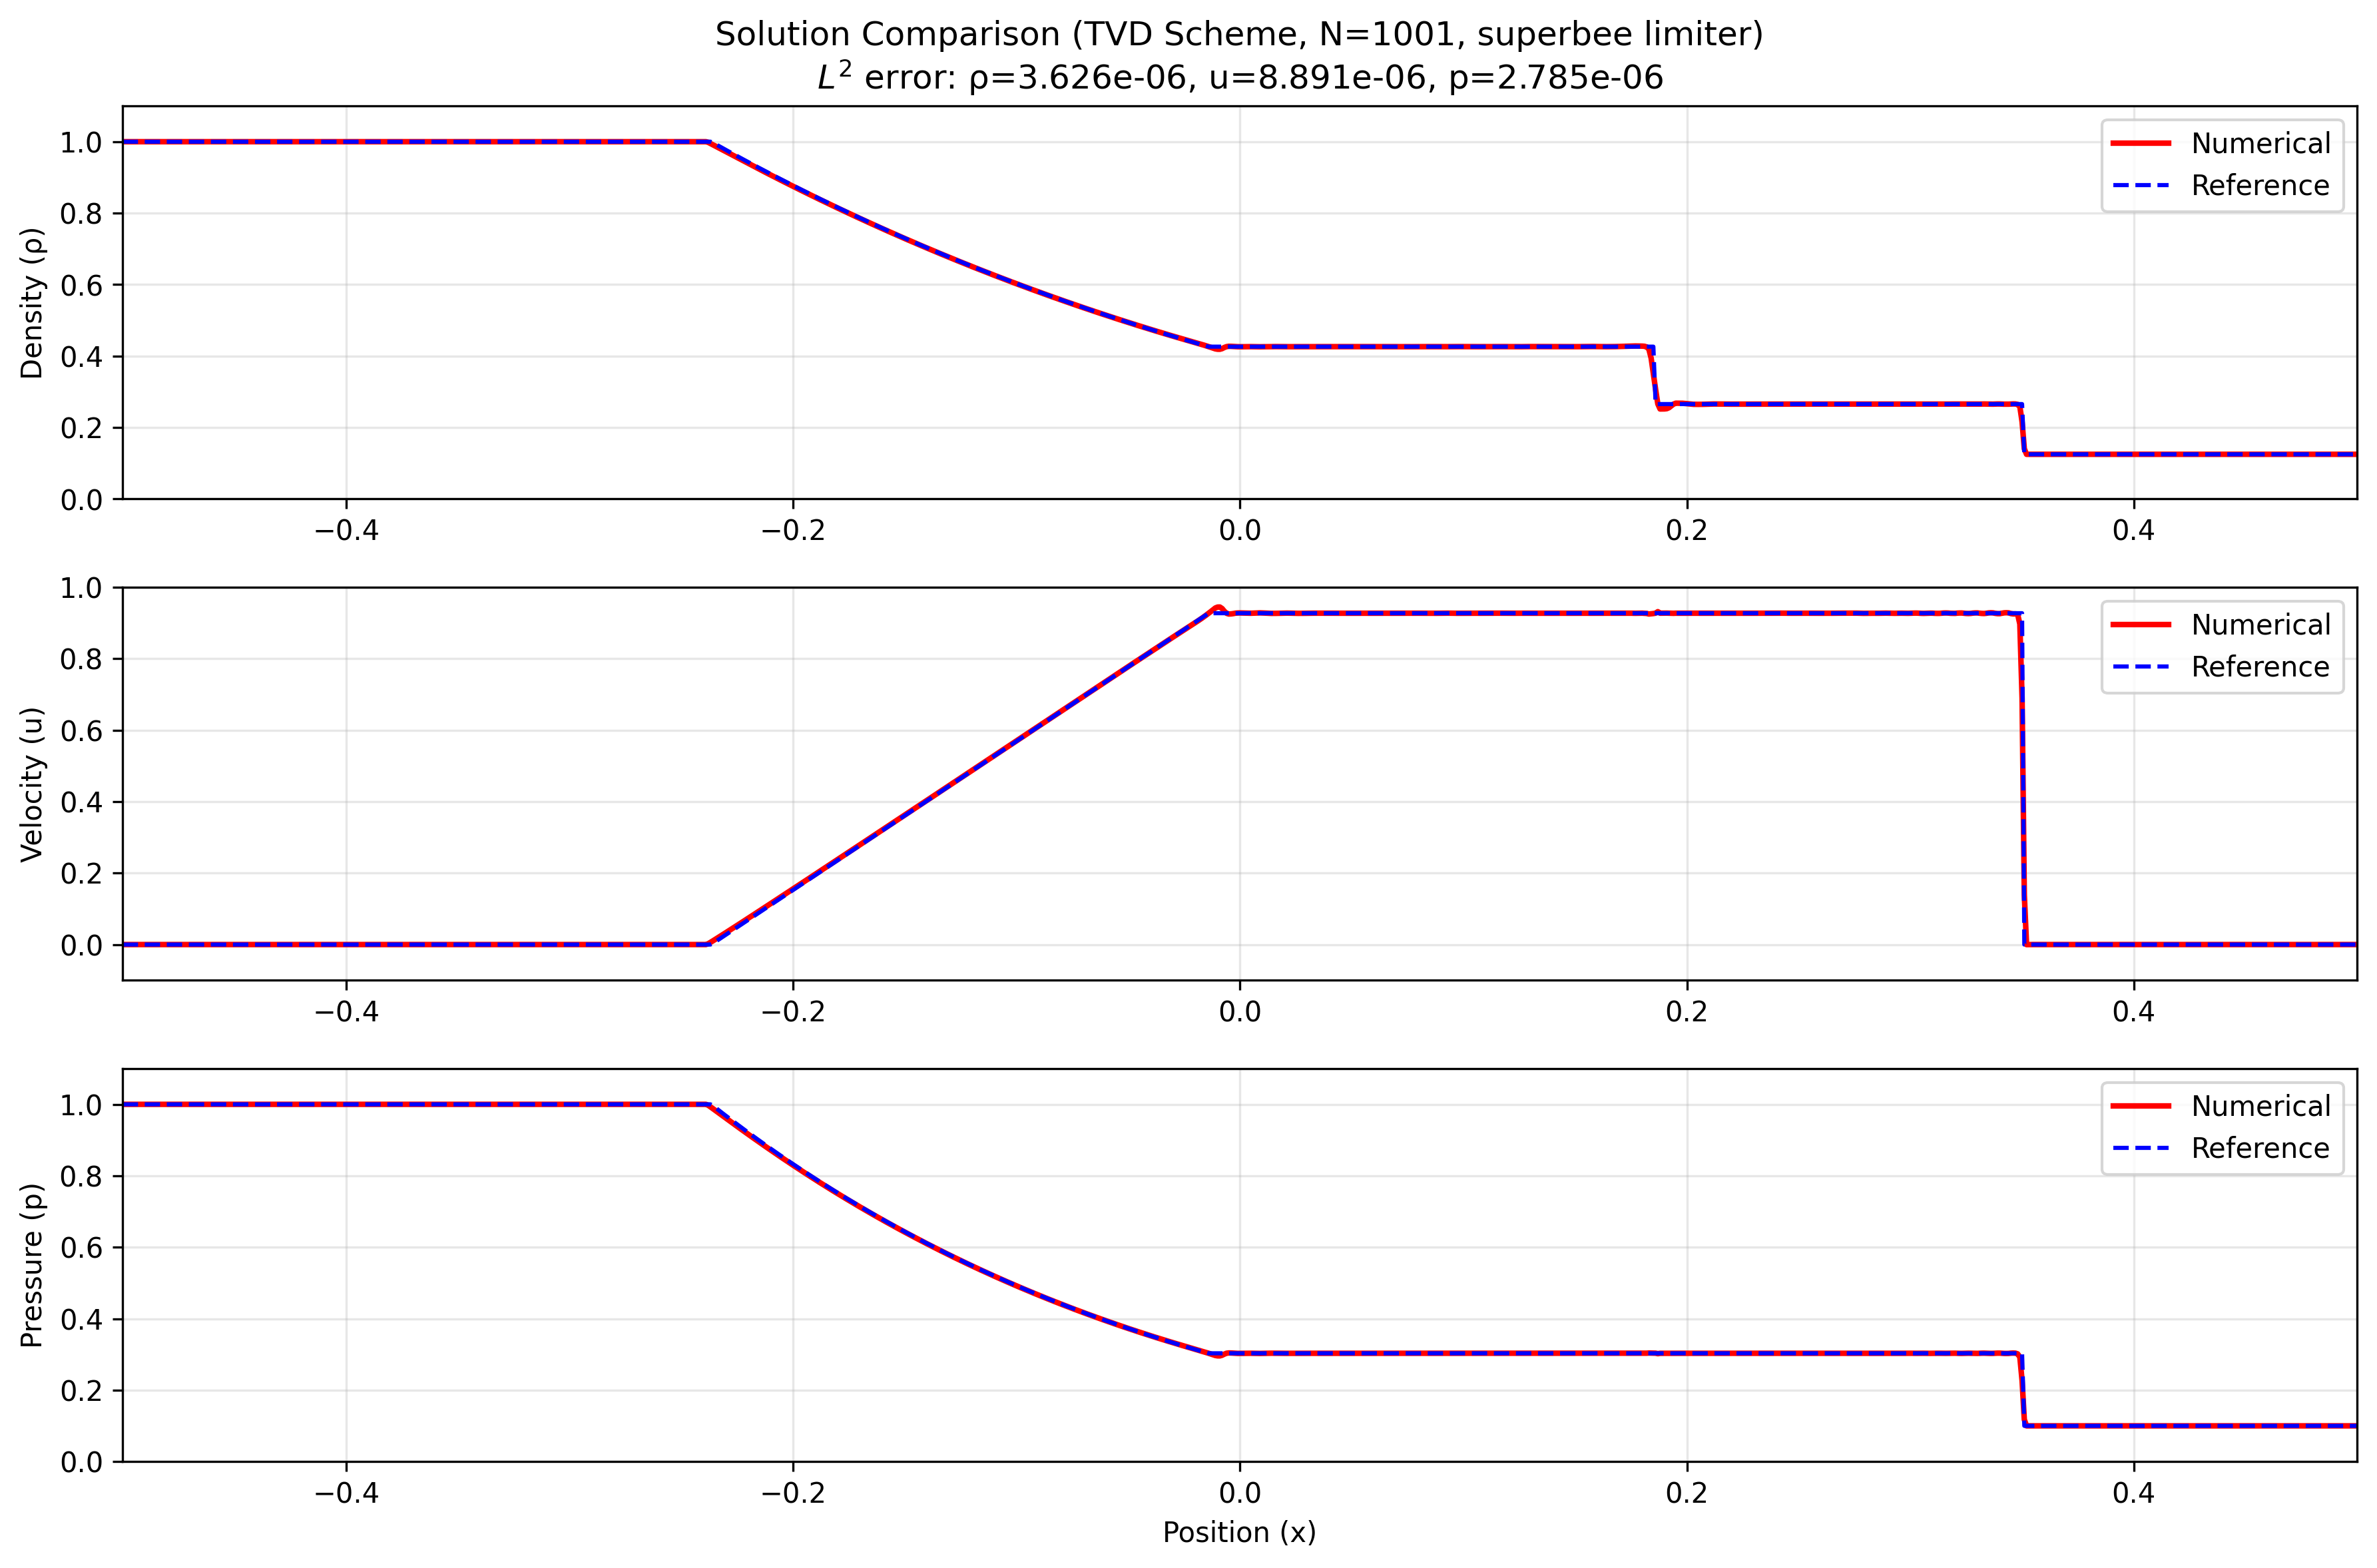
\includegraphics[width=\textwidth]{./pictures/Solution Comparison (TVD Scheme, N=1001, superbee limiter).png} 
        \caption{Superbee限制器}
    \end{subfigure}
    \vspace{0.5cm}
    \centering
    \begin{subfigure}[b]{0.45\textwidth} 
        \centering
        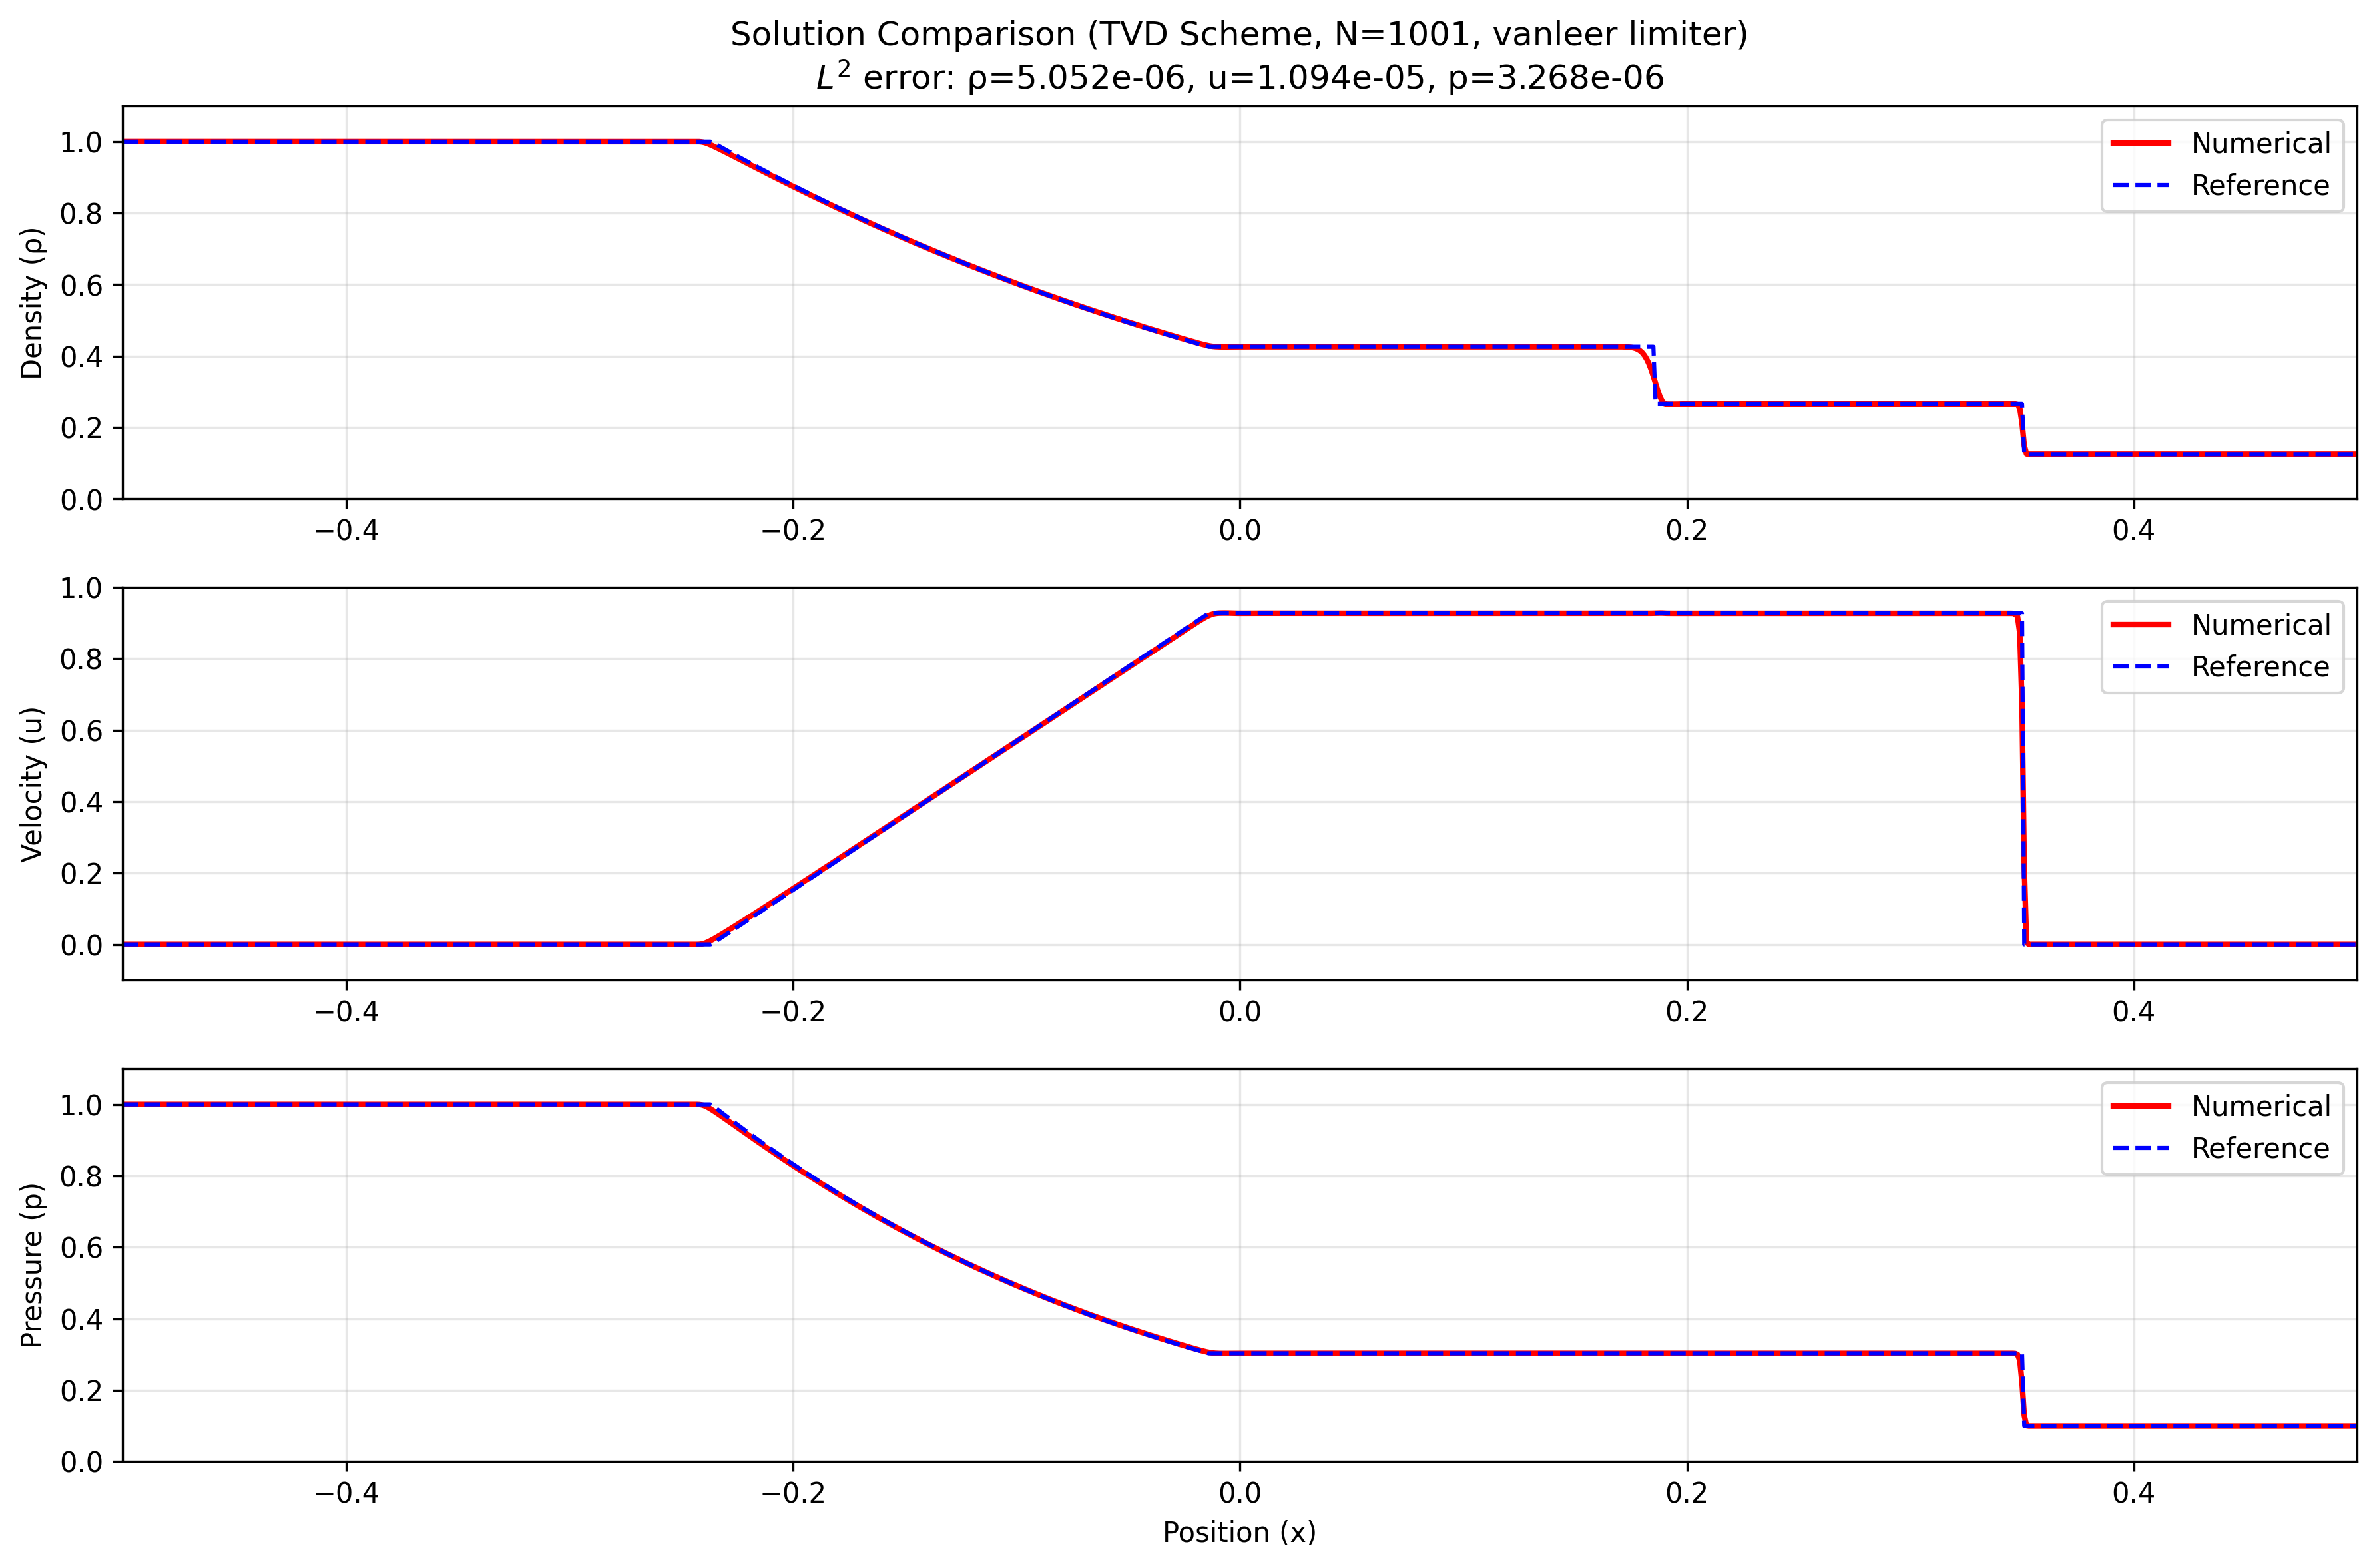
\includegraphics[width=\textwidth]{./pictures/Solution Comparison (TVD Scheme, N=1001, vanleer limiter).png} 
        \caption{Van Leer限制器}
    \end{subfigure}
    \caption{TVD格式选用不同限制器的计算结果}
\end{figure}

可以看出,以L2误差衡量,Superbee限制器效果最好,但在间断及导数间断处有轻微振荡现象。对于激波捕捉精度,Van Leer限制器稍好于Minmod限制器。Minmod限制器的稳定性较强,在计算剧烈的间断时仍具有稳定性,但对应的缺陷是在极值点处的精度下降。

\section{NND格式计算结果}
NND格式计算结果如图3所示。
\begin{figure}[htbp]
    \centering
    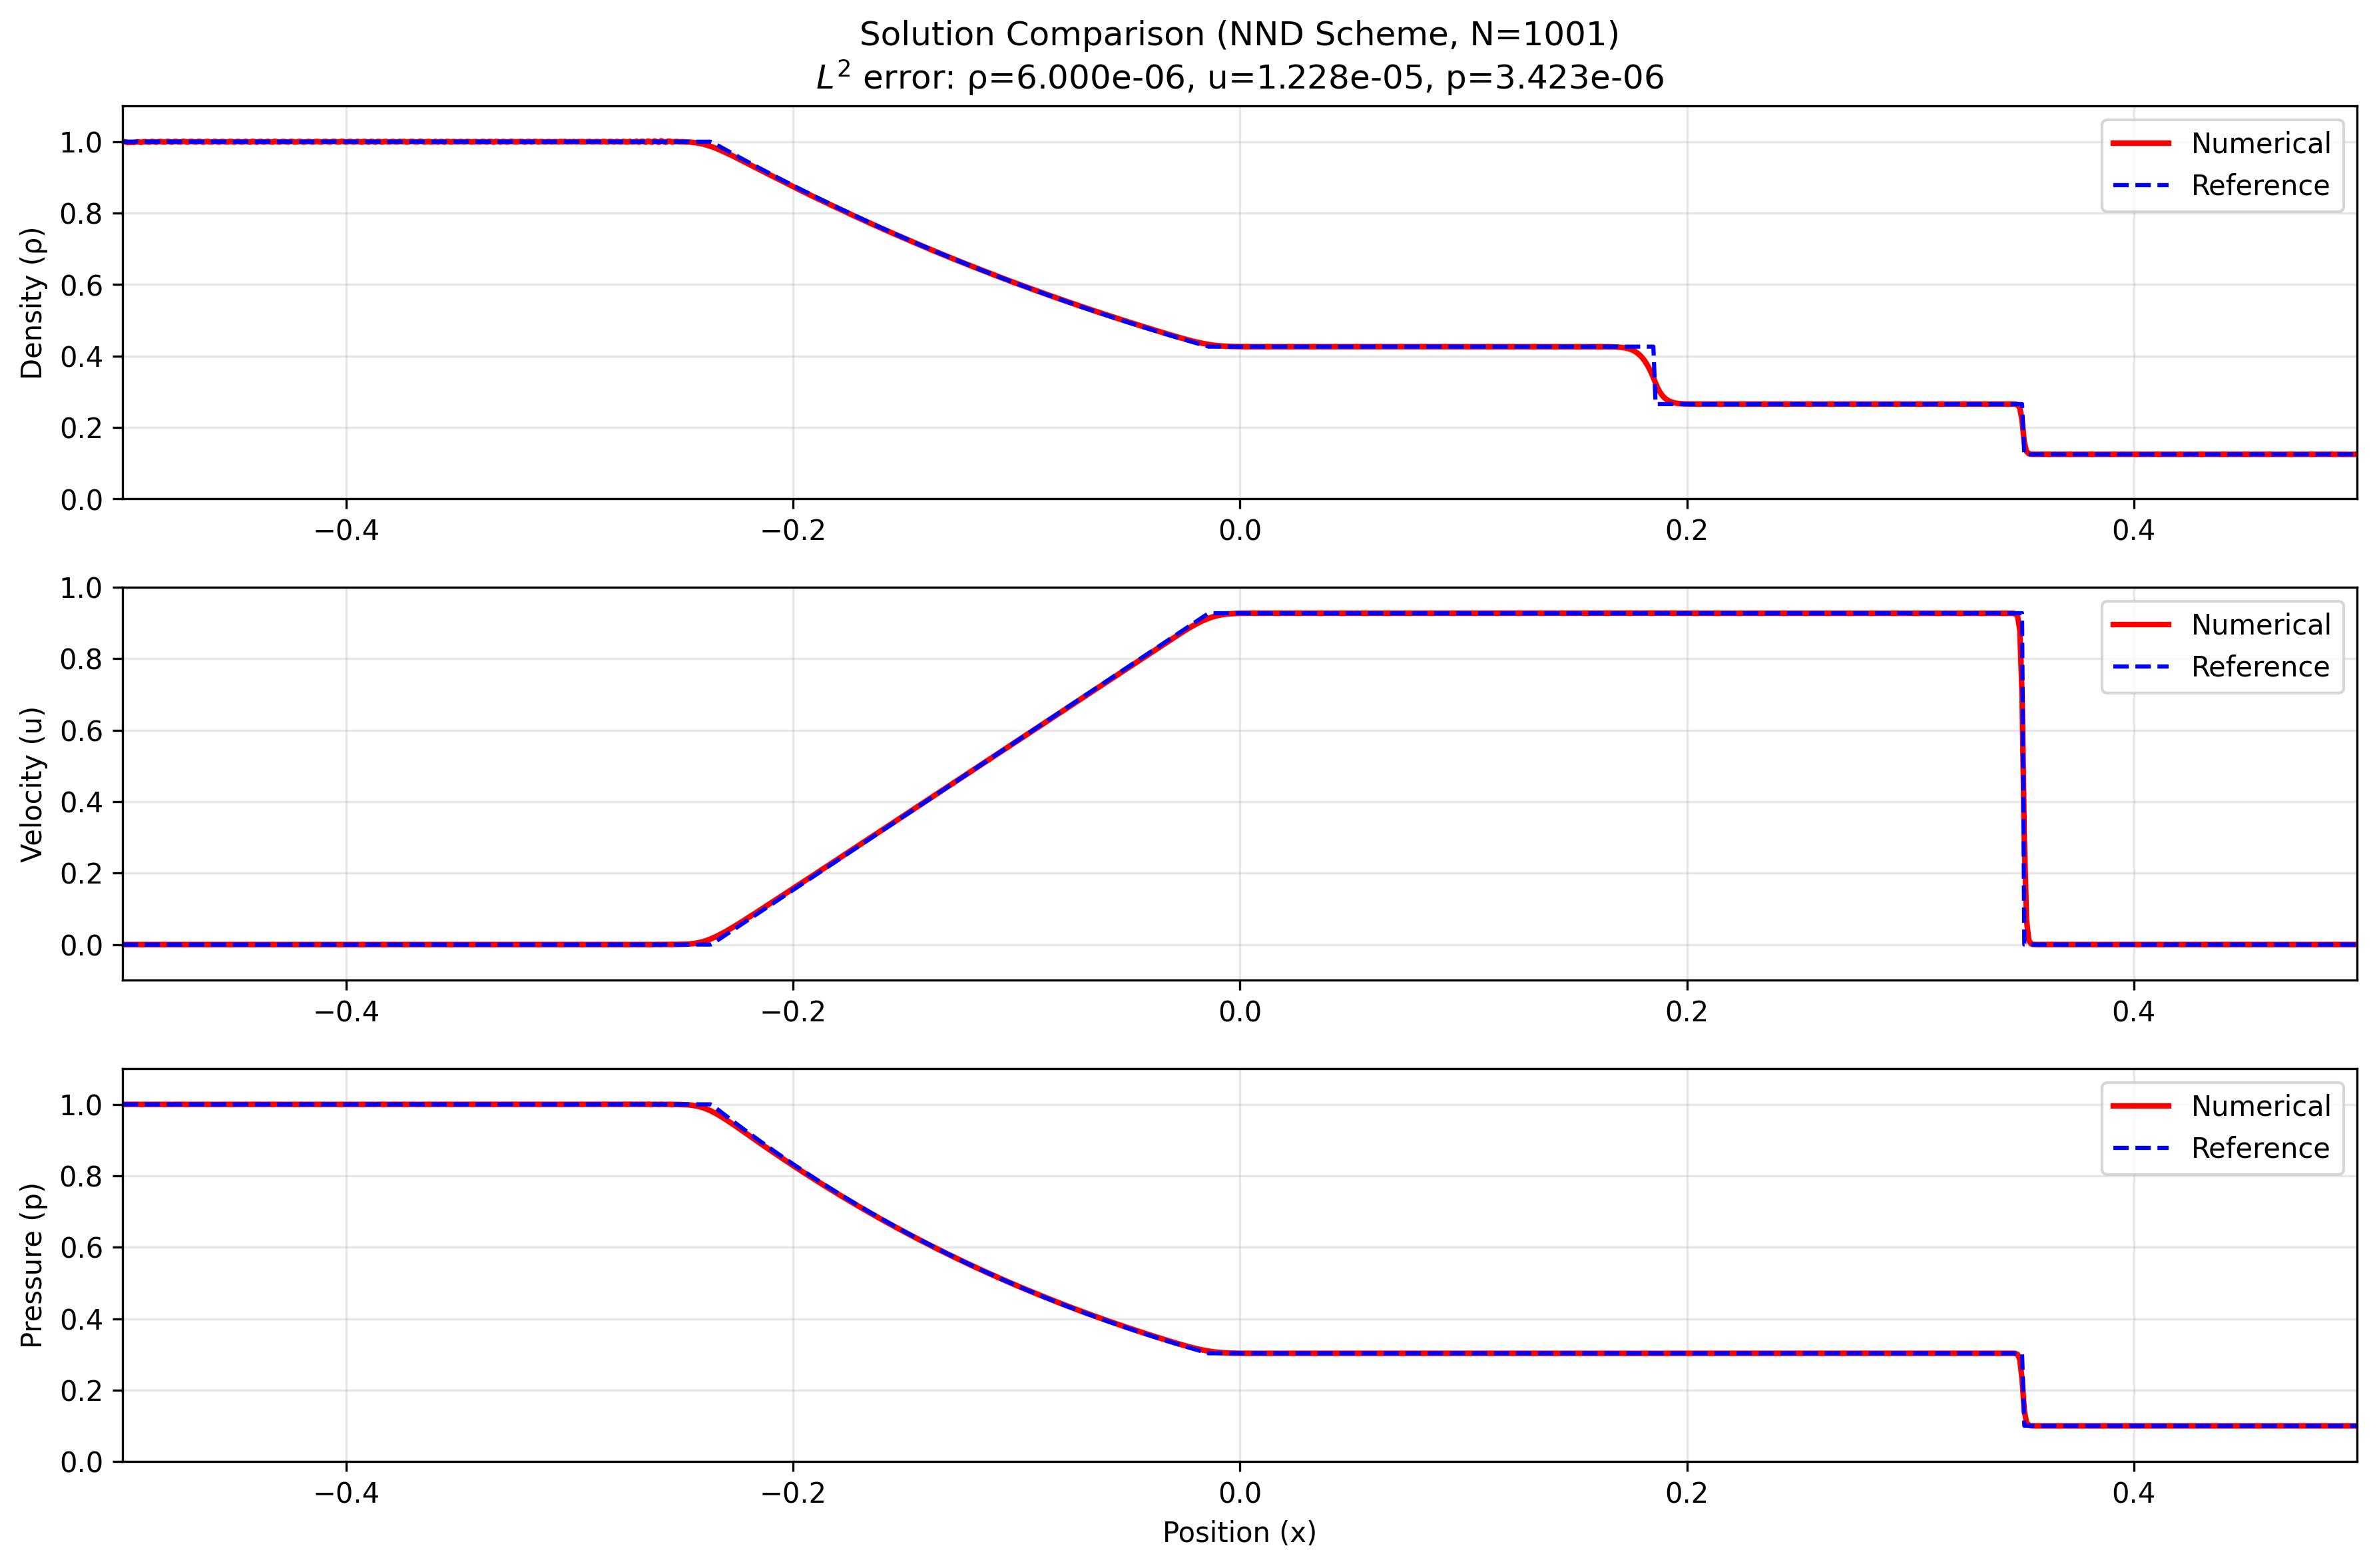
\includegraphics[width=0.45\textwidth]{./pictures/Solution Comparison (NND Scheme, N=1001).png}
    \caption{NND格式计算结果}
\end{figure}

从计算结果和误差来看,NND格式均与采用Minmod限制器的TVD格式一致。这说明了二者本质上是不同视角下的同种格式。

\section{WENO格式计算结果}
图4是采用原理讨论中两种不同的光滑度量时WENO格式的计算结果。
\begin{figure}[htbp]
    \centering
    \begin{subfigure}[b]{0.45\textwidth} 
        \centering
        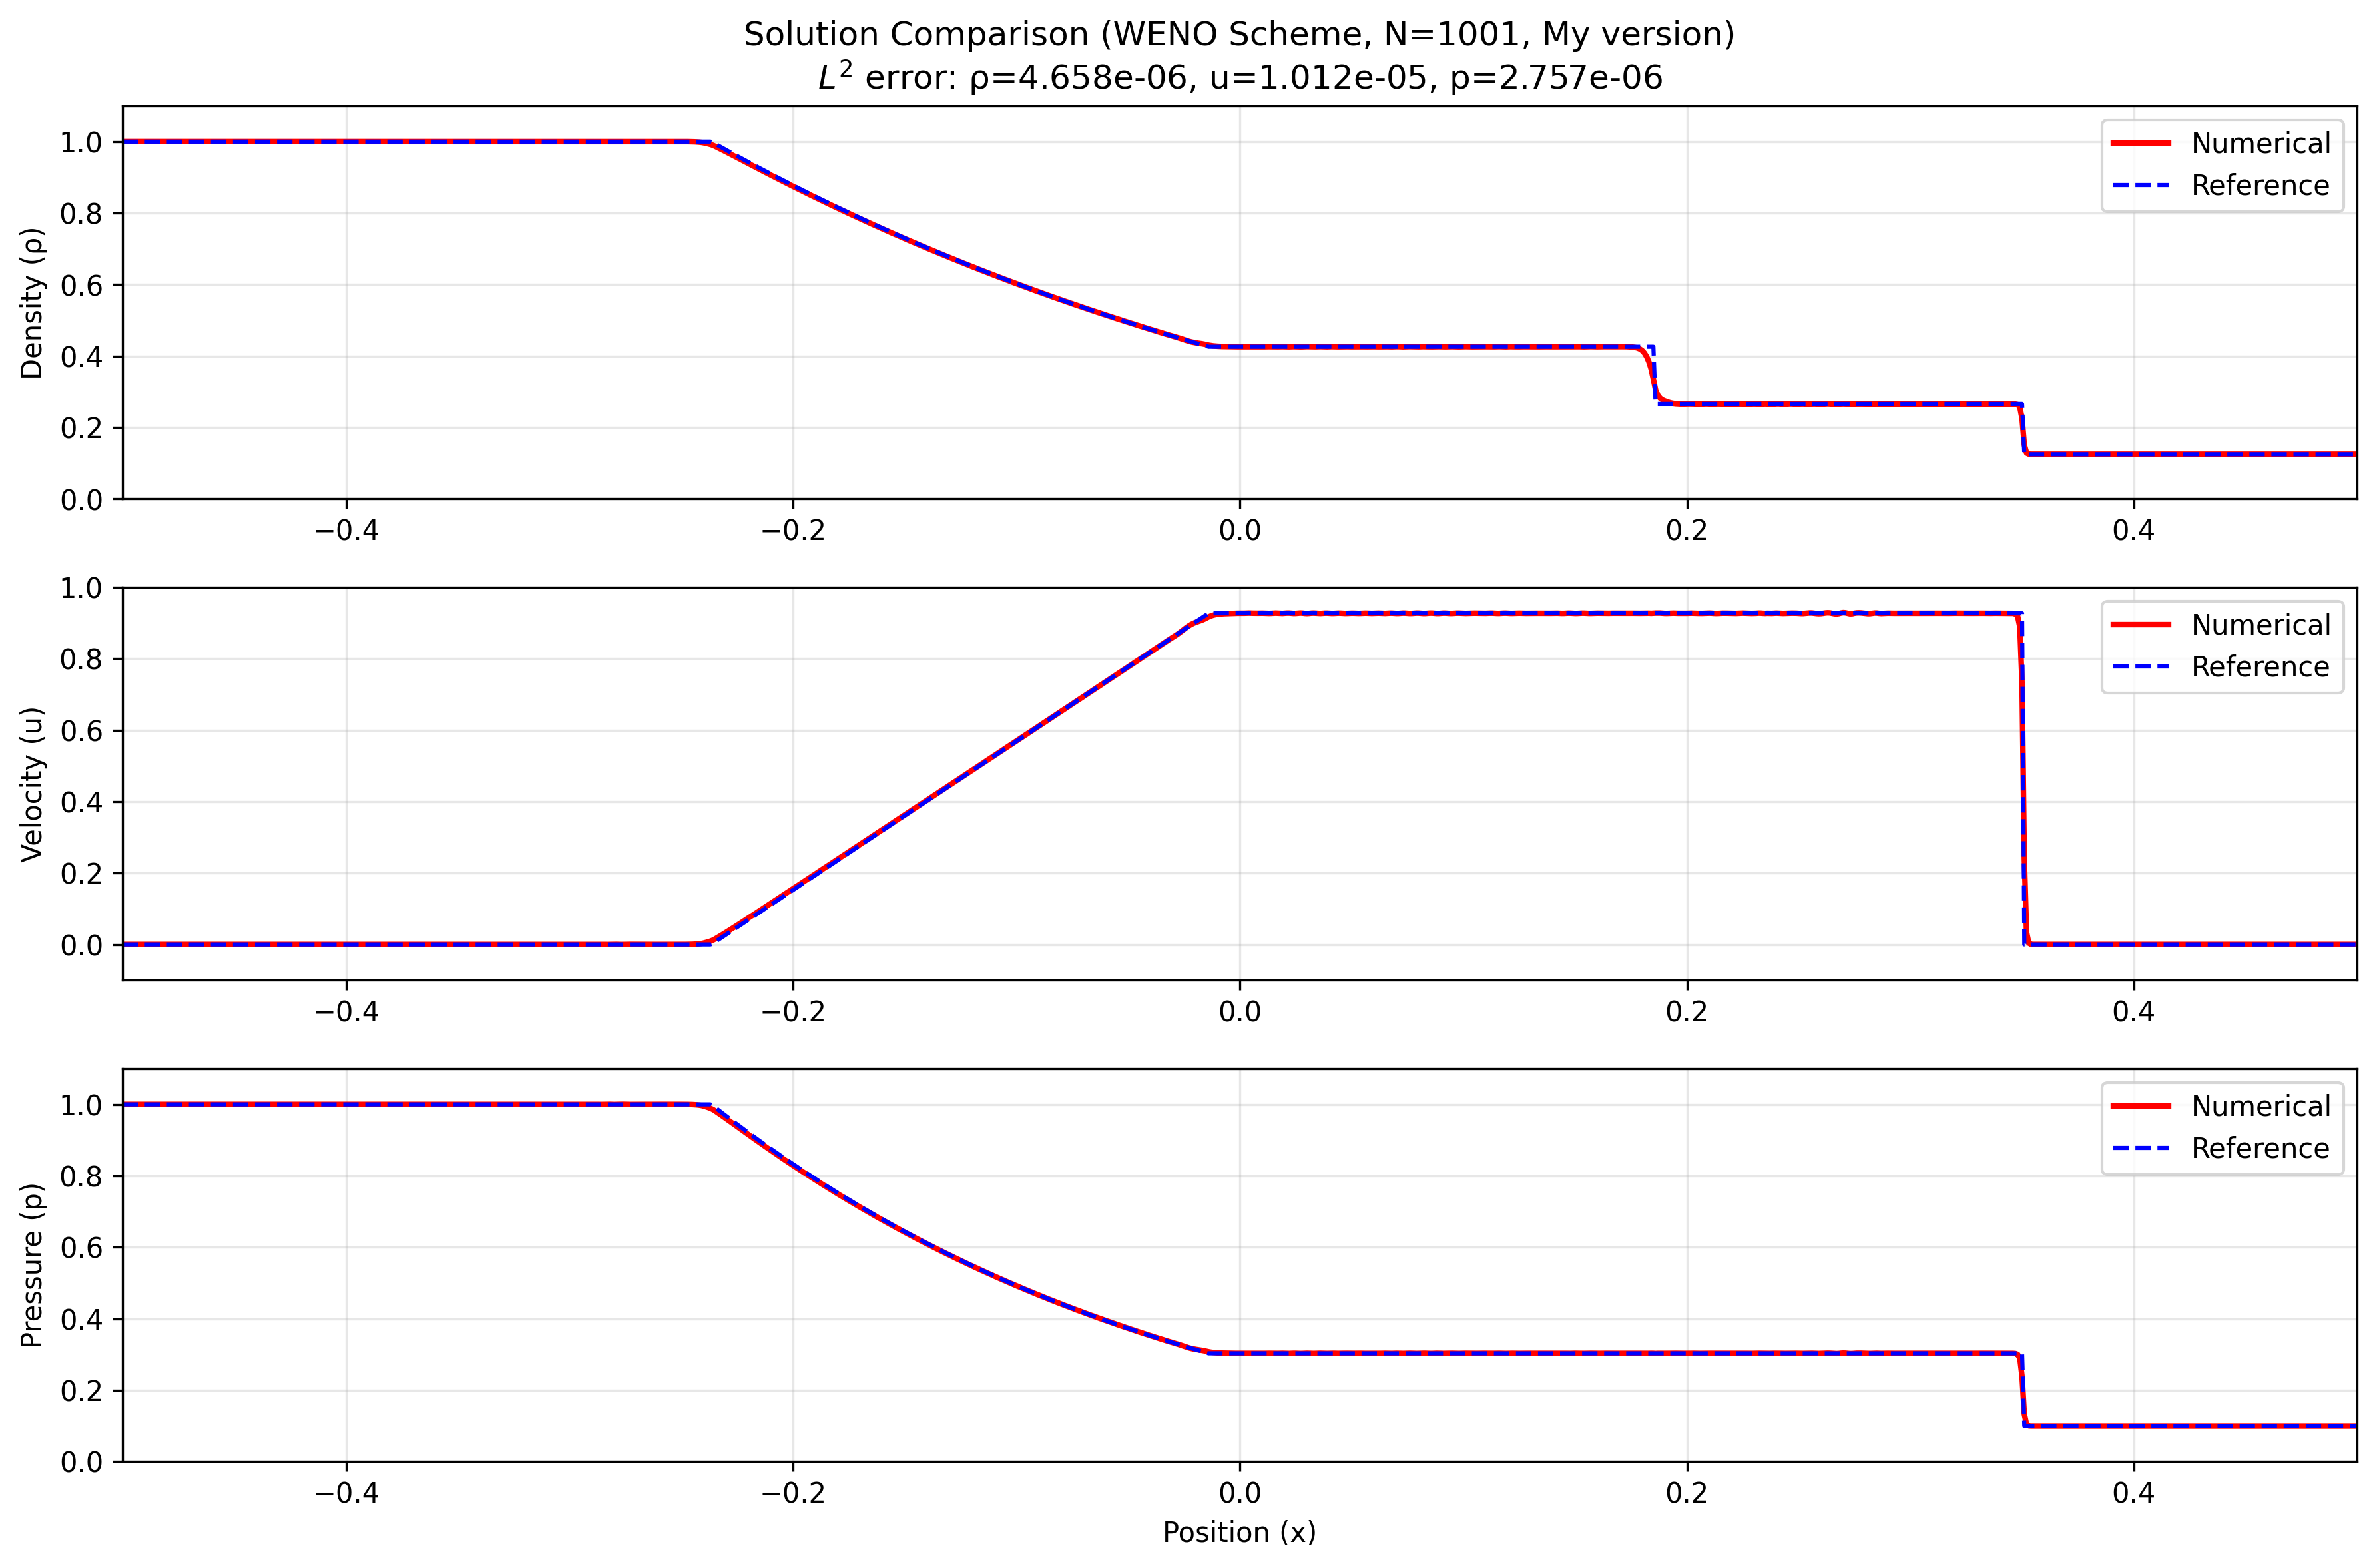
\includegraphics[width=\textwidth]{./pictures/Solution Comparison (WENO Scheme, N=1001, My version).png} 
        \caption{以全部差分格式的平方和作为光滑度量}
    \end{subfigure}
    \hfill
    \begin{subfigure}[b]{0.45\textwidth} 
        \centering
        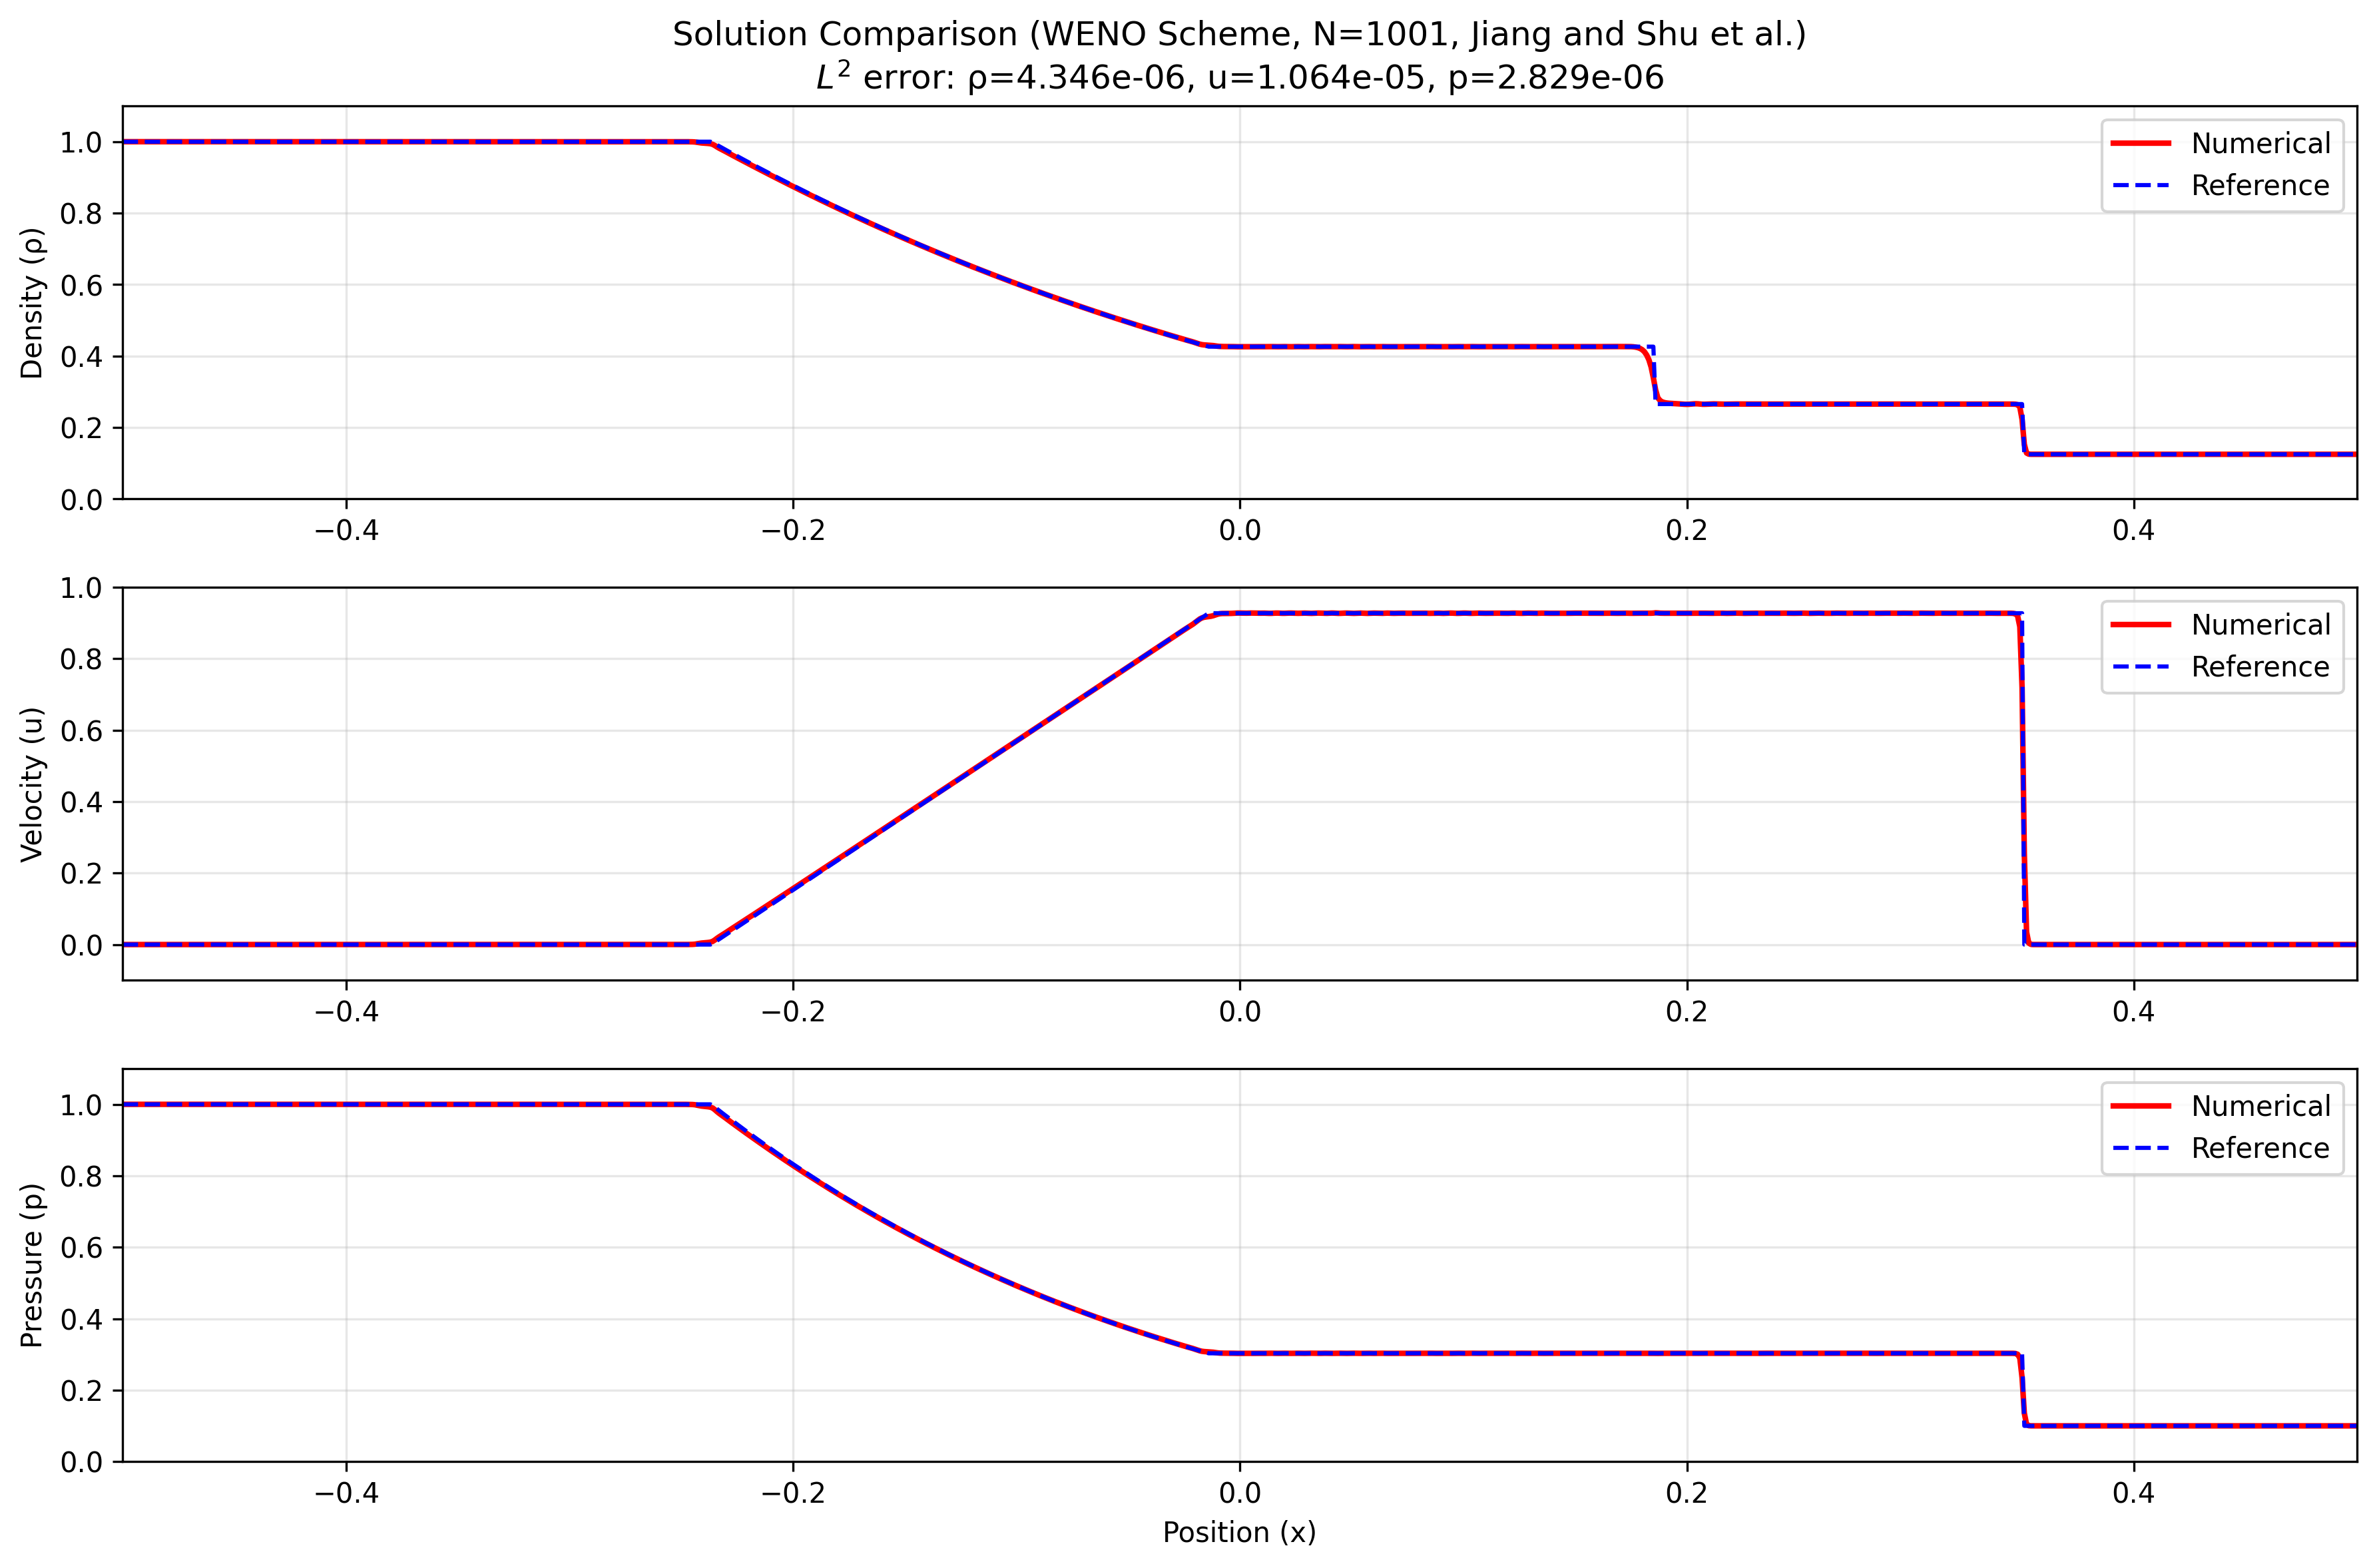
\includegraphics[width=\textwidth]{./pictures/Solution Comparison (WENO Scheme, N=1001, Jiang and Shu et al.).png} 
        \caption{WENO5经典光滑度量}
    \end{subfigure}
    \vspace{0.5cm}
    \caption{采用不同光滑度量的WENO格式计算结果}
\end{figure}

可以看出,二者在Sod激波管问题中的L2误差基本一致。然而,理论上说常用的WENO5光滑度量应该具有更高阶的精度。结合Sod激波管问题来看,这应当是由于有大量格点导数为0,在这些格点处区分不出二者精度的差异。这使得二者计算结果的误差相差不大。

\section{采用特征重构法的WENO格式计算结果}
在WENO格式中加入特征重构方法,得到的计算结果如图5所示。
\begin{figure}[htbp]
    \centering
    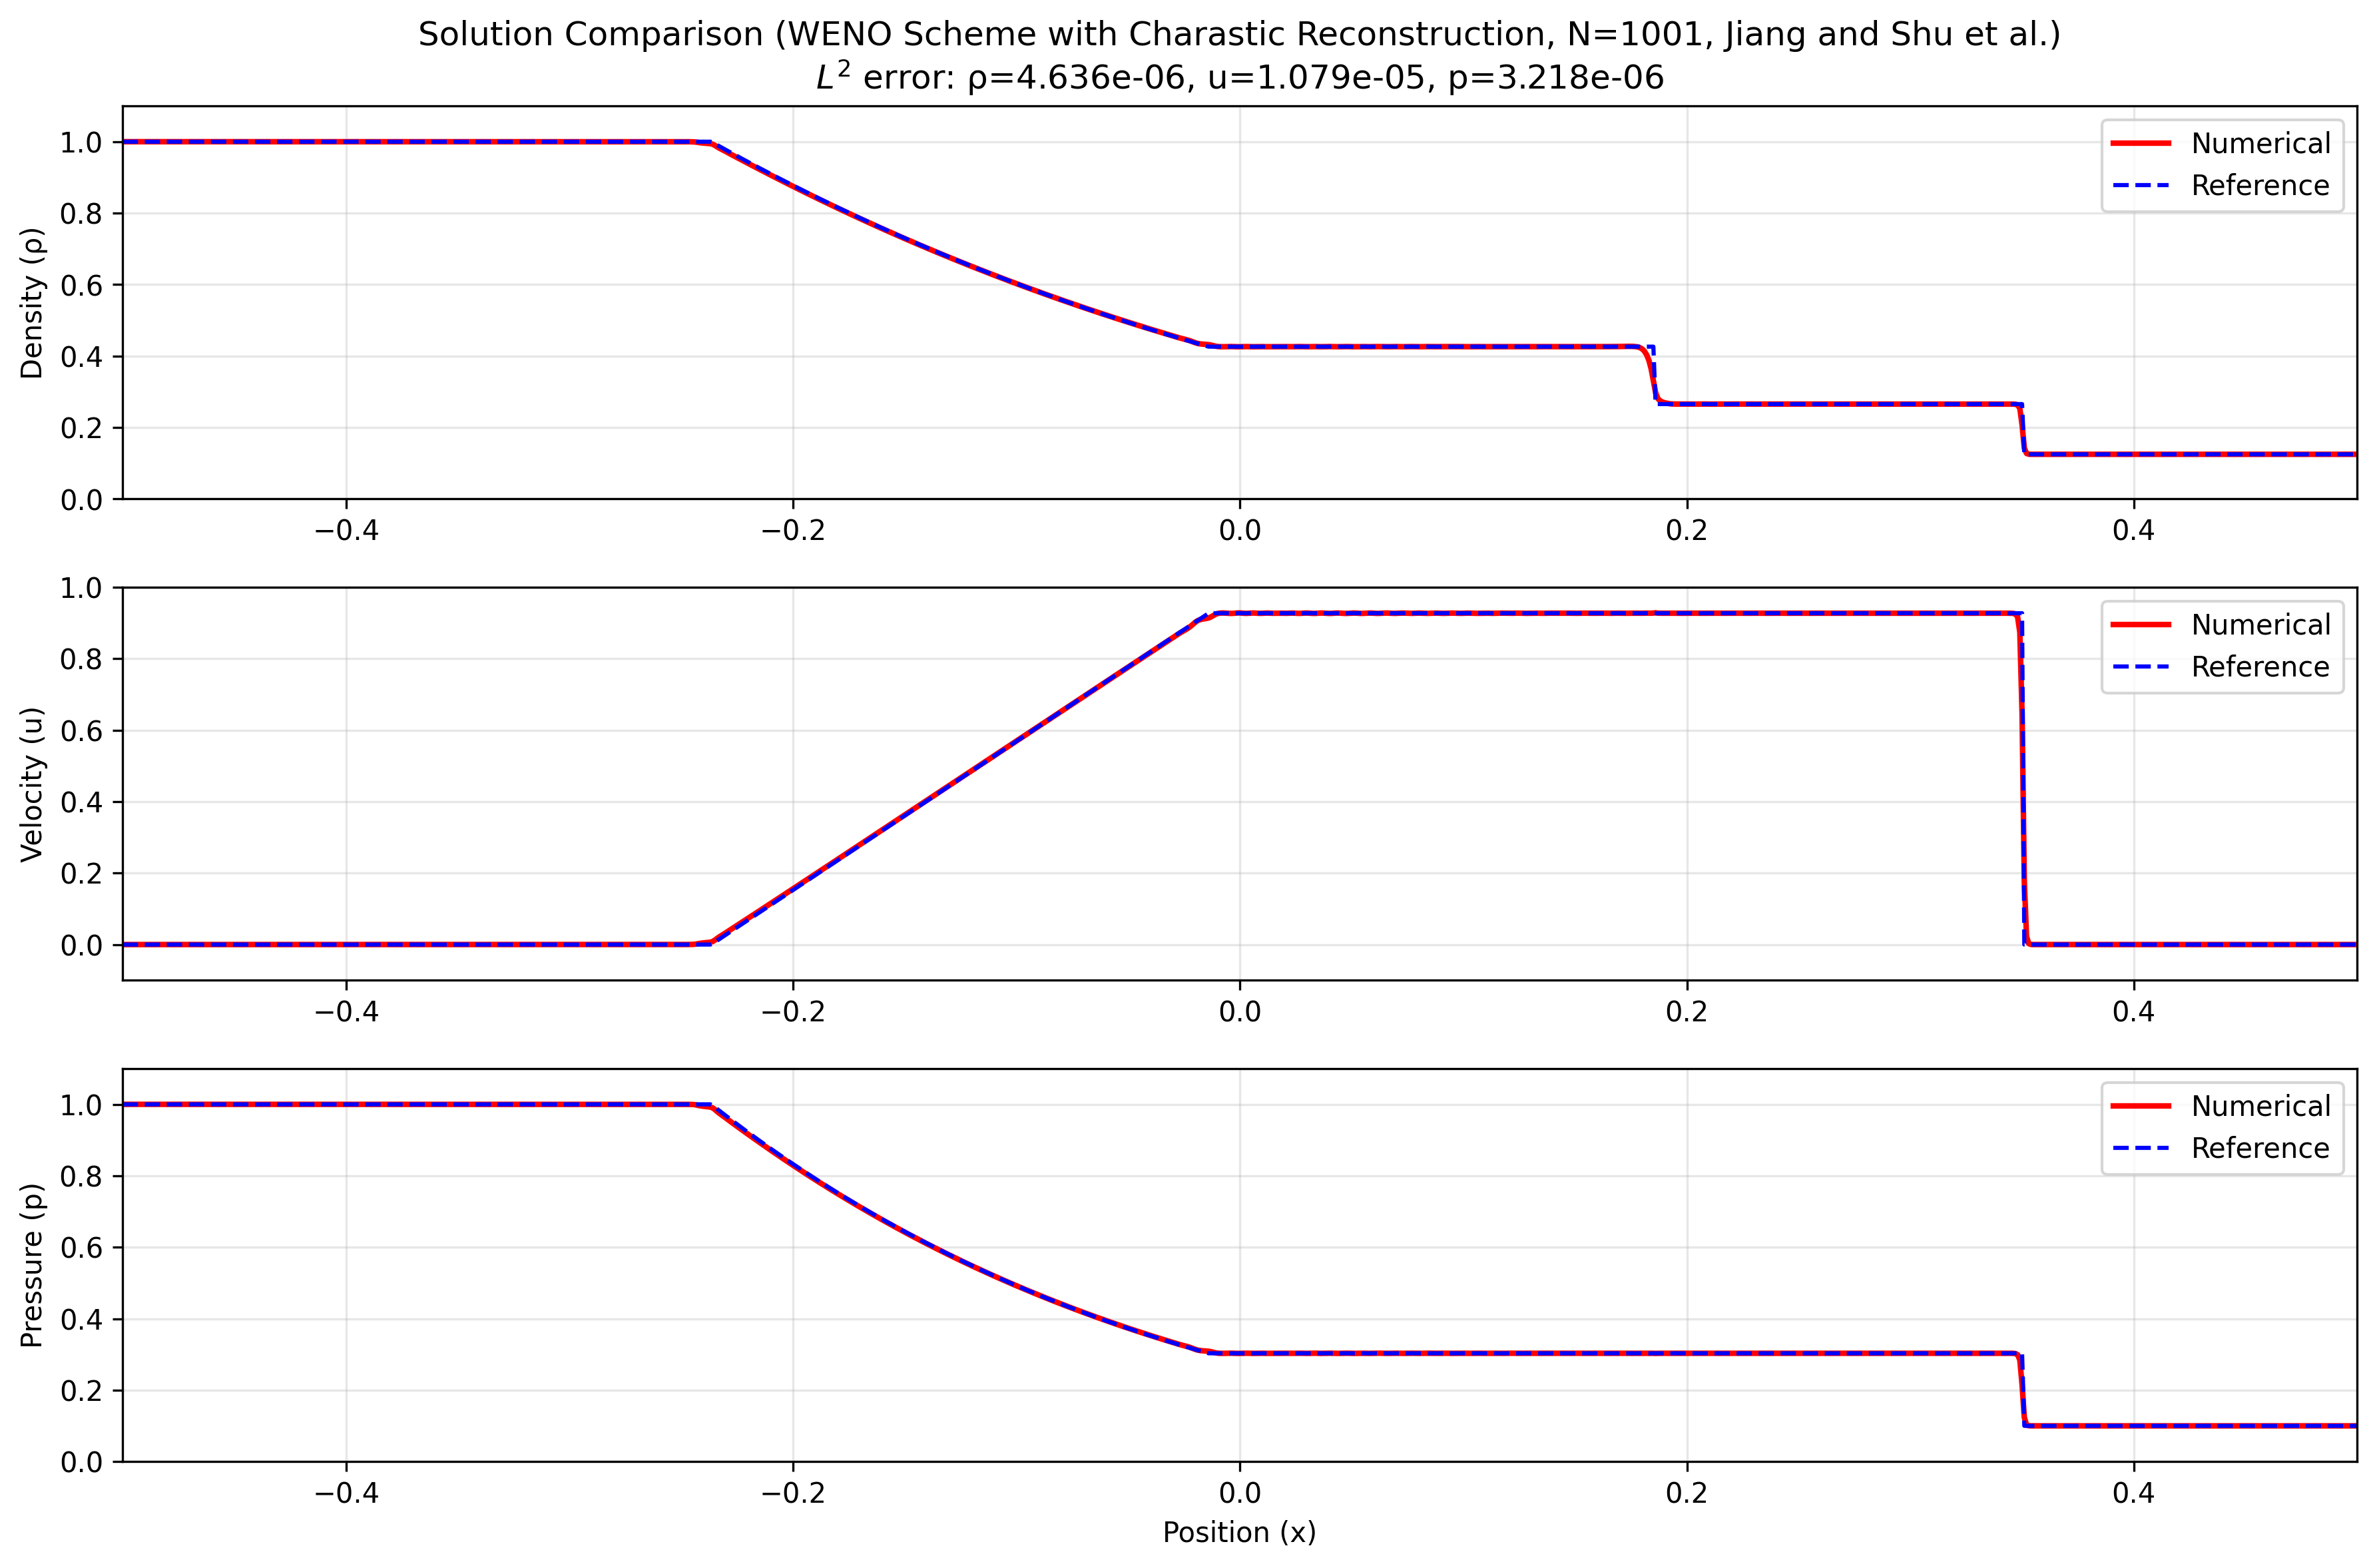
\includegraphics[width=0.45\textwidth]{./pictures/Solution Comparison (WENO Scheme with Charastic Reconstruction, N=1001, Jiang and Shu et al.).png} 
    \caption{采用特征重构法的WENO格式}
\end{figure}
与图4中的计算结果一致。特征重构法的好处是,在特征空间计算数值通量的物理意义更加明确,计算更加稳定。

\section*{附1:AI工具使用说明表}
使用的AI工具:deepseek和GPT-4o

AI生成代码行数及功能:numerical\_test.py中98-138,443-496行由AI生成,前者用于计算Roe矩阵的绝对值对角化,后者为画图功能。

核心代码自主编写比例:83\%

\section*{附2:git版本控制记录}
\begin{figure}[htbp]
    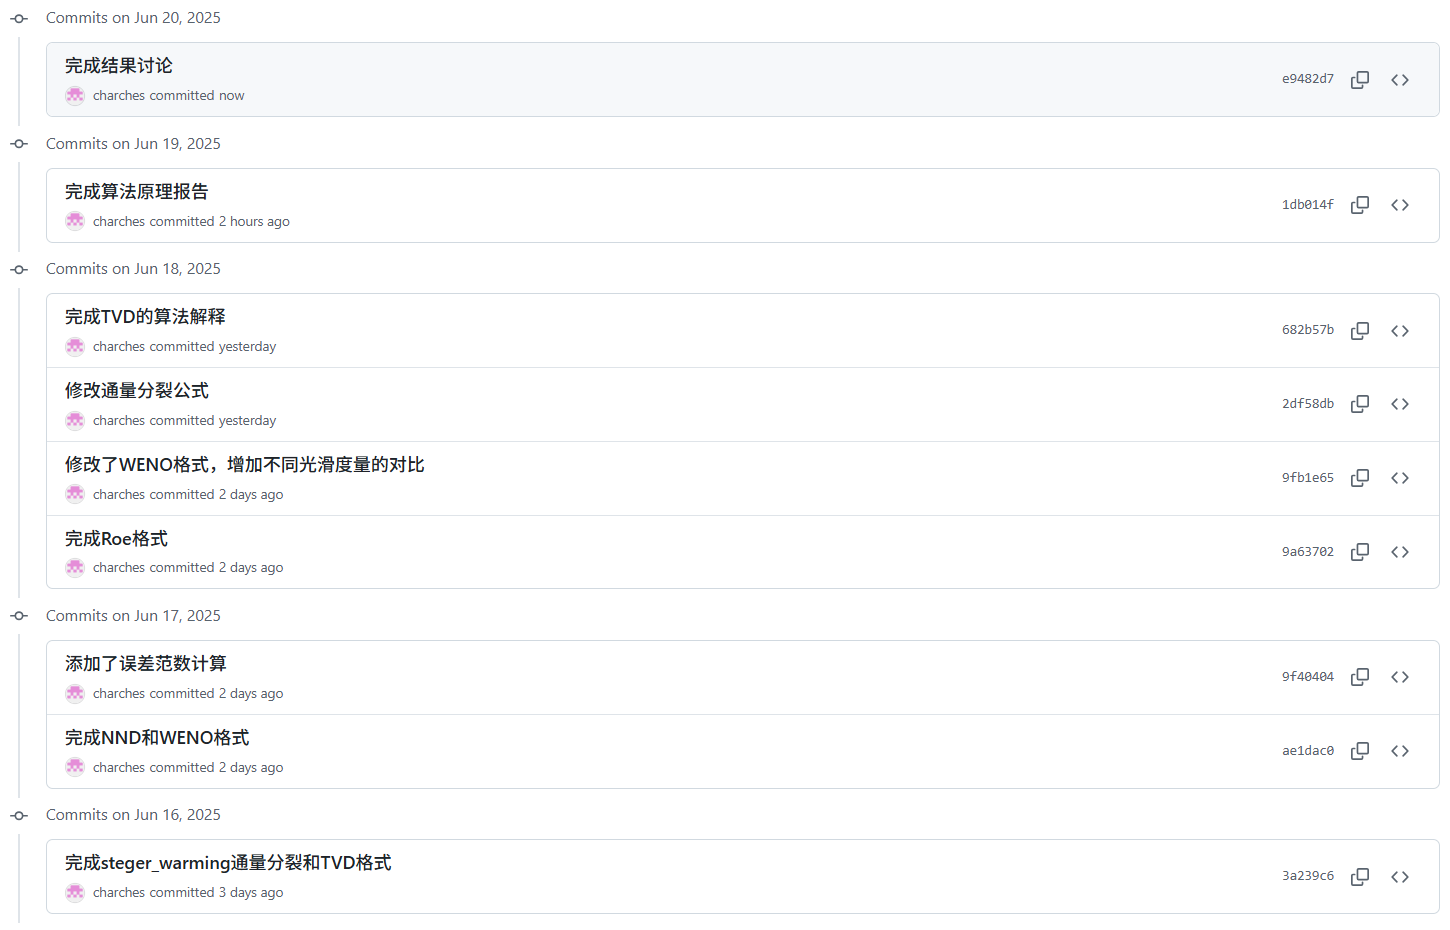
\includegraphics[width=0.8\textwidth]{./pictures/git_control.png}
\end{figure}
\end{document}